\documentclass[12pt,a4paper]{scrreprt}

\usepackage[latin1]{inputenc}   % UNIX Umlaute und �
%\usepackage{ae}                 % interne 8bit Codierung f�r bessere Trennungen
\usepackage[ngerman]{babel}           % deutsche Trennungen und Bezeichnungen
%\usepackage{bibdbis}            % Literaturangaben aus der Datenbank mit bibtex
\usepackage{amsmath,amsfonts,amssymb}
\usepackage {natbib}
\citestyle{dinat}
\usepackage{typearea}           % Satzspiegelberechnung: Texth�he und -breite
\typearea{12}                   % je h�her das Argument, desto kleiner die R�nder
\usepackage{graphicx}           % zur Graphikeinbindung
\usepackage{amssymb,amsmath}	% mathematische Symbole
\usepackage{color}
\usepackage{picins} 					%Bilder umflie�en
\usepackage{multicol}
\usepackage{placeins}					%Gleitobjekte erzwingen \FloatBarrier 					
\usepackage{pifont}  					%Symbole
\usepackage{listings} \lstset{numbers=left, numberstyle=\tiny, numbersep=5pt} \lstset{language=XML}


\usepackage{pdftricks}			% Zeichnen von B�umen
%\begin{psinputs}
%\usepackage{pst-all}
%\end{psinputs}			
\setcounter{secnumdepth}{3} %Gibt an wieviele Ebenen nummeriert werden
%% ... und nimm alle 4 Ebenen in das Inhaltsverzeichnis auf.
\setcounter{tocdepth}{3}
\addtolength{\topmargin}{.5cm}  	% Rand oberhalb der Kopfzeile
%\setlength{\footskip}{1.2cm}		% Abstand Text - Fusszeile
%\oddsidemargin+13mm					% R�nder f�r ungerade Seiten
%\addtolength{\evensidemargin}{-2cm}	% R�nder f�r gerade Seiten
\textheight24cm						% Vertikale Texth�he

\parskip3mm						%Abstand zwischen Abs�tzen
\parindent0mm					%Einr�ckung bei Absatzbeginn


\newcommand{\hidden}[1]{}
\newcommand{\code}[1]{{\tt #1}}
\newcommand{\relation}[1]{\textsc{#1}}
\newcommand{\attrib}[1]{\textit{#1}}
\newcommand{\lsemijoin}{\ltimes}
\newcommand{\rsemijoin}{\rtimes}
\newcommand{\lantisemijoin}{\: \overline{\ltimes}}
\newcommand{\rantisemijoin}{\: \overline{\rtimes}}
% \newcommand{\fullouterjoin}{\sqsupset\hspace{-2.1mm}\times\hspace{-2.1mm}\sqsubset}
\newcommand{\element}{\in}
\newcommand{\notelement}{\;|\hspace{-2ex}\in}
\newcommand{\cbox}[2]{\parbox{#1}{\begin{center} #2 \end{center}}}

\newenvironment{iterator}[1]{\begin{minipage}{15.2cm}\textbf{iterator} #1 \\}
{\end{minipage}}
\newenvironment{method}[1]{\hspace*{0.2cm}\textbf{#1}\begin{itemize}}{\end{itemize}}
\newenvironment{subproc}{\begin{itemize}}{\end{itemize}}
\newenvironment{costtable}{\begin{center}\renewcommand{\arraystretch}{1.5}\begin{tabular}{l|c|c}}{\end{tabular}\end{center}}
\newenvironment{formtable}[1]{\begin{center}\renewcommand{\arraystretch}{2}\begin{tabular}{#1}}{\end{tabular}\end{center}}
\newtheorem{Def}{Definition}

\date{\today \\[2cm]
	Erstpr�fer: Prof. Dr. Kurt Schneider\\
	Zweitpr�fer: \\
	Betreuer: Dipl.-Wirt.-Inform. Daniel L�bke}
\author{Alex Salnikow\\
		Matr.Nr. 2116853\\[1cm]
		}
\title{ \vspace*{-3cm}
		{
		\normalsize\textsc{Fachgebiet Software Engineering\\
		Institut f�r Praktische Informatik\\
		Fachbereich Informatik\\
		Universit�t Hannover}\\[1cm]
		}
	%	\hrule Horizontale Linie
		\vspace*{4cm}
		{\Huge Masterarbeit} \\
		{\large im Studiengang Informatik} \\[1cm]
		{\Huge Ermittlung von Testabdeckungsmetriken}\\
		{\Huge in BPEl-Komositionen}\\[1cm]}



\begin{document}
%\maketitle			
%\thispagestyle{empty}
\vspace*{10cm}
\huge{Eidesstattliche Erkl�rung}\vspace{2cm}

\normalsize{Hiermit versichere ich, Alex Salnikow, die vorliegende Masterarbeit ohne fremde Hilfe und
nur unter Verwendung der von mir aufgef�hrten Quellen und Hilfsmittel angefertigt zu haben.\vspace{2cm}

Hannover, \today  \ \ \ \ \ \ \ \ \ \ \ \ \ \ \ \ \ \ \ \ \ \ \ \ \ \ \ \ \ \ \ \ \ \ \ \ \ \ \ \ \ \ \ \ \ \ ............................\\

}


\begin{titlepage}
\begin{center}
\vspace*{1cm}
		{
		\normalsize\textsc{\textbf{Gottfried Wilhelm Leibniz Universit�t Hannover\\
Fakult�t f�r Elektrotechnik und Informatik\\
Institut f�r Praktische Informatik\\
Fachgebiet Software Engineering}}\\[2.5cm]
		}
		
		\huge{\textbf{
		Ermittlung von Testabdeckungsmetriken\\
		in BPEL-Kompositionen}}\\[3cm]
		
		\Large{\textbf{Masterarbeit}}\\[0.5cm]
\large{im Studiengang Informatik\\[0.5cm]
von}\\[0.5cm]
\Large{\textbf{Alex Salnikow}}\\[3.5cm]

\large{\textbf{Pr�fer: Prof. Dr. Kurt Schneider\\
Zweitpr�fer: Prof. Dr.-Ing. Gabriele von Voigt\\
Betreuer: Dipl.-Wirt.-Inform. Daniel L�bke}\\[1cm]
Hannover, \today}
\end{center}
\end{titlepage}	
%\vspace{1cm}
%\newpage
%\thispagestyle{empty}
%{\Large \bf Zusammenfassung}
\thispagestyle{empty} 
\vspace*{5cm}
\begin{center}
\textbf{Zusammenfassung}
\end{center}

Business Process Execution Language (BPEL) hat sich in der Industrie als Mittel f�r die Kombination der Web Services zu einem Prozess etabliert. Die dabei abgebildeten Gesch�ftsprozesse sind f�r das Unternehmen sehr wichtig. Demzufolge haben die Korrektheit und die Robustheit der BPEL-Prozesse sehr hohe Priorit�t, was ein gr�ndliches Testen der Prozesse notwendig macht. Allerdings gibt es f�r BPEL noch keine praktischen Metriken, die f�r die Bewertung der Testqualit�t oder Testfortschritts geeignet sind. In dieser Arbeit werden Testabdeckungsmetriken aus der klassischen Softwareentwicklung (Statement- und Zweigabdeckung) auf BPEL �bertragen und entsprechend angepasst. Zus�tzlich werden BPEL-spezifischen Metriken eingef�hrt, die die wichtigen Eigenschaften der Sprache gesondert ber�cksichtigen. Anschlie�end wird die Erweiterung des BPELUnit-Frameworks pr�sentiert, die einfache Sammlung und Pr�sentation der Metriken erm�glicht. Mit dieser Erweiterung k�nnen die Tester einfach und schnell den Fortschritt und die Qualit�t ihrer Arbeit kontrollieren.  


%\vspace{1cm}
  
\parskip0mm
\newpage
%\thispagestyle{empty}~
\pagenumbering{arabic}
\tableofcontents
\parskip5mm
\chapter{Einleitung}
\section{Motivation}
Unternehmen sehen sich heute mit sehr dynamischen M�rkten konfrontiert und sind 
einem starken internationalen Wettbewerb ausgesetzt. Zu den Anforderungen solcher
M�rkte geh�ren oft flexible Gesch�ftsprozesse. Die notwendige Anpassungsf�higkeit der
Unternehmen und deren Gesch�ftsprozessen h�ngt meistens direkt von der vorhandenen
IT-Infrastruktur ab. Um diesen Anforderungen gerecht zu werden, muss die Softwarearchitektur
daf�r sorgen, dass IT-Systemen zum einen an den Gesch�ftsprozessen ausgerichtet
sind, zum anderen sehr einfach bei Ver�nderungen angepasst werden k�nnen. 
Eine m�gliche L�sung, die zur Zeit von vielen bevorzugt wird, sind Serviceorientierte Architekturen und Web Service Standards. 

Die Funktionen werden bei solchen Architekturen in Services gekapselt, die in Kompositionen zu vollautomatischen Gesch�ftsprozessen verkn�pft werden. F�r die Realisierung der Kompositionen steht mit WS-BPEL ein OASIS-Standard zu Verf�gung, der durch Unterst�tzung vieler wichtiger Softwarehersteller auf dem Weg zu einem Industriestandard ist. Damit �bernimmt BPEL  eine Schl�sselfunktion innerhalb der Konzeption einer serviceorientierten Architektur.

Die entscheidende Rolle der BPEL-Prozessen innerhalb eines Unternehmens erfordert hohe Qualit�tssicherung. Aufgrund der relativen Neuheit des ganzen Technologiebereichs gibt es auf diesem Gebiet noch wenige Erfahrungen.
Obwohl einige Konzepte und L�sungen f�r das systematische Testen von BPEL-Kompositionen bereits erarbeitet und umgesetzt wurden, wurden viele Methoden, die sich in der konventionellen Softwareentwicklung bew�hrt haben, noch nicht f�r BPEL angepasst. Die Testabdeckung, die im Zusammenhang mit Qualit�tssicherung der Software eine sehr wichtige Rolle spielt, z�hlt zu den Themen, die im BPEL-Kontext noch nicht behandelt wurde. 

Unter Testabdeckung versteht man Metriken f�r das Verh�ltnis zwischen zu testenden und tats�chlich getesteten Elementen des Pr�flings (in diesem Fall einer BPEL-Komposition). Diese Metriken werden  oft als Indikatoren f�r die Qualit�t und Fortschritt der Tests verwendet. Es fehlen f�r BPEL bislang sowohl Definitionen der Metriken als auch Verfahren zur Ermittlung der Testabdeckung. Diese Masterarbeit besch�ftigt sich mit genau diesen Themen.

Aus praktischer Sicht ist die Integration der Testabdeckungsmetriken in ein Test-Werkzeug besonders sinnvoll. Mit dem schnellen Zugriff auf die erreichten Testabdeckungswerte ist st�ndige und unmittelbare Kontrolle der Testqualit�t m�glich. Im praktischen Teil dieser Arbeit wird das BPELUnit-Framework, das das Testen von BPEL-Kompositionen unterst�tzt, erweitert. Als Ergebnis eines Tests soll das Framework neben der Aussage, ob der Test erfolgreich war oder nicht, auch die erreichte Testabdeckung liefern. 




\section{Aufgabenstellung}
In dieser Arbeit werden die Testabdeckungsmetriken f�r BPEL-Prozesse formal definiert. Dabei werden die bekannten Metriken (Anweisungs- und Zweigabdeckung) auf BPEL-Kompositionen �bertragen und neue BPEL-spezifische Metriken bestimmt, die die wichtigen Eigenschaften der Sprache abdecken. Die Metriken werden so gestaltet, dass die 100\% Abdeckung, was theoretisch optimal ist, bei jedem BPEL-Prozess erreichbar ist. 

Es werden Verfahren f�r die Ermittlung der Abdeckungsmetriken in BPEL-Kompositionen vorgestellt und bewertet. Unter Ber�cksichtigung des ausgew�hlten Verfahrens werden Konzepte zur Ermittlung der Metriken vorgestellt.

Als Realisierung wird im praktischen Teil dieser Arbeit das BPELUnit-Framework erweitert und die zugeh�rigen Clients angepasst. Einfache Konfigurationsm�glichkeit, die Transparenz der Testabdeckungsmessung und detaillierte und verst�ndliche Ergebnisdarstellung stehen dabei im Vordergrund. 
 
\section{Aufbau der Arbeit}
  
\chapter{Grundlagen}
\section{SOA}
Die Unternehmen sind heutzutage an agilen IT-Systemen interessiert, die die Gesch�ftsprozesse unterst�tzen und flexibel auf Ver�nderungen reagieren k�nnen.  
Serviceorientierte Architekturen (SOA) verspricht diese F�higkeit zur effektiven und flexiblen Unterst�tzung sich immer schneller �ndernder Gesch�ftsprozesse. 
  
  SOA ist ein Ansatz zum Entwurf verteilter Systeme. \textit{Die Kernidee der SOA, die Unternehmensfunktionalit�t
als Menge voneinander unabh�ngiger Dienste zur Verf�gung
zu stellen, bildet die Basis f�r Integration und Dynamik} \cite{THOMAS2005}. Eine m�gliche Definition f�r SOA:
\begin{quotation}
\begin{Def}\textit{Eine serviceorientierte Architektur ist ein
Konzept f�r eine Systemarchitektur, in
welchem Funktionen in Form von wiederverwendbaren, voneinander unabh�ngigen
und lose gekoppelten Services implementiert
werden. Services k�nnen unabh�ngig von
zugrunde liegenden Implementierungen �ber
Schnittstellen aufgerufen werden, deren
Spezifikationen �ffentlich sind. Serviceinteraktion
findet �ber eine daf�r vorgesehene
Kommunikationsinfrastruktur statt.}
\cite{WikiSOA}
\end{Def}
\end{quotation}

  Die Funktionen einer Anwendung sind als Services organisiert, die 
 beliebig verteilt sein k�nnen und sich dynamisch zu Gesch�ftsprozessen verbinden lassen. Die zugrunde liegenden technischen Plattformen der einzelnen Services spielen dabei keine Rolle. Zu betonen ist, dass SOA eine Systemarchitektur und keine Technologie beschreibt. 

 
\section{Web Services}
%Web Services sind aktuell die wichtigste Realisierung einer SOA und werden in der Software Industrie anerkannt. Mittlerweile setzen viele gro�e Softwarekonzerne auf Web Services und haben ihre Produktstrategien entsprechend ausgerichtet.

Als Web-Service bezeichnet man im Allgemeinen eine Softwarekomponente, die
ihre Funktionalit�at �uber Standardinternetprotokolle zur Verf�ugung stellt.
W3C definiert die Web Services folgenderma�en: 
\begin{Def}
A software application identified by a URI, whose interfaces and bindings are capable of being
defined, described, and discovered as XML artifacts. A Web service supports direct interactions
with other software agents using XML-based messages exchanged via Internet-based protocols.(W3C)
\end{Def}

a.) Ein Web Service wird durch einen URI identifiziert.1
b.) Die Schnittstelle eines Web Services ist maschinenlesbar und wird durch
WSDL (siehe n�chsten Abschnitt) beschrieben.
c.) Ein Web Service kommuniziert mit anderen Softwarekomponenten durch
XML Nachrichten. Der Nachrichtenaustausch kann insbesondere mit Hilfe
von Internetprotokollen (z.B. HTTP oder SMTP) stattfinden.

W�hrend die erste Definition die Eigenschaften von Web Services beschreibt,  die zweite Definition auf die wichtigen Standards ein. 
\begin{Def}
A Web service is a software system designed to support interoperable machine-to-machine
interaction over a network. It has an interface described in a machine-processable format
(specifically WSDL). Other systems interact with the Web service in a manner prescribed by its
description using SOAP messages, typically conveyed using HTTP with an XML serialization in
conjunction with other Web-related standards (W3C 2004a).
\end{Def}

Gem�� der beiden Definitionen sind die Beschreibung von Schnittstellen und
der Nachrichtenaustausch wesentliche Aufgaben. SOAP, WSDL und UDDI sind die daf�r vorgesehen Standards und bilden den Kern der Web Services.
\begin{itemize}
	\item SOAP ein standardisiertes, XML-basiertes
Protokoll zum Verpacken von Nachrichten, die zwischen Applikationen ausgetauscht
werden. setzt SOAP
auf die Netzwerk- und Transportschichten auf. Es ist also irrelevant, welche
Transportmechanismen f�ur den eigentlichen Versand verwendet werden.Die gebr�auchlichste Form des Austausches von SOAP-Nachrichten ist die �Ubertragung
�uber HTTP.
\item UDDI
dient zur Lokalisierung und Ver�ffentlichung
von Web-Services im Internet
UDDI = Register f�r Diensteund ihre Beschreibungen+ Suchmethoden+ Publishingmethoden
UDDI-Daten enthalten Kontakt-Informationen, Listen von Business Services und Infos, wie einService via Protokoll angesprochen werden kann
Um einen Web-Service im Internet zu finden, ist ein Verzeichnisdienst notwendig.
F�ur diese Zwecke wurde der Universal Description, Discovery and Integration-
Standard geschaffen. UDDI bietet Standardfunktionen zum Klassifizieren,
Katalogisieren und Verwalten von Daten und Metadaten �uber Web-
Services, so da� diese einfach gefunden und verwendet werden k�onnen.
\item WSDL (Web Services Defnition Language) ist eine funktionale, XML-basierte Beschreibungssprache
f�r die Schnittstellen eines Web Services.(siehe n�chsten Abschnitt)
\end{itemize}

\begin{figure}[htbp]
	\centering
		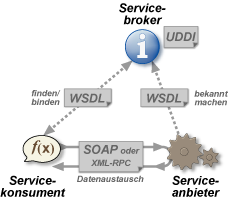
\includegraphics{bilder/Webservice.png}
		\caption{Kontrollfluss eines BPEL Prozesses}
	\label{fig:ExamlpleBPELProzess}
\end{figure}

Bei Web Services handelt es sich nicht um eine bestimmte Technik, sondern um ein B�ndel von verschiedenen Standards und Spezifikationen.
Web Service Stack ...

Bild

Im n�chsten Abschnitt wird WSDL etwas genauer vorgestellt.


\subsection{SOAP}
\subsection{WSDL}
\section{Komposition der Services mit BPEL}
\subsection{Partner}
%WS-BPEL(kurz BPEL) ist eine XML-basierte, ausf�hrbare Sprache zur Modellierung und Beschreibung
von Gesch�ftsprozessen. BPEL ist 2002 aus IBMs WSFL und Microsofts XLANG entstanden und liegt aktuell in der Version 2.0  als OASIS Standard vor. Durch breite Produktunterst�tzung ist die Sprache auf dem Weg, sich auch als Industriestandard zu etabliert.


Mit BPEL l�sst sich ein Prozess beschreiben, der verschiedene Web Services zu einer Gesamtanwendung verkn�pft. Services k�nnen dabei auf zwei Arten kombiniert werden:
\begin{itemize}
	\item \textbf{Orchestration:} Ein zentraler Prozess koordiniert die
Operationen der Web Services, die in den Prozess
eingebunden sind.
\item \textbf{Choreography:} Es gibt keinen zentralen Koordinator. Jeder in
die Choreography eingebundene Web Service kennt seine Interaktionspartner. Bei der Choreographie erfolgt
die Zusammenarbeit �ber den Austausch von Nachrichten
in einem �ffentlichen Prozess.
\end{itemize}

BPEL unterst�tzt Orchestration und Choreography durch
\begin{itemize}
	\item \textbf{Executable Processes:} Spezifikation des intenen Verahaltens eines
Ge\-sch�fts\-pro\-zesses, der durch eine Engine
ausgef�hrt werden kann. Enth�lt alle f�r die Pro\-zess\-aus\-f�h\-rung notwendige Informationen bis auf die tats�chlichen Endpunkte der Web Services.
\item \textbf{Abstract Business Processes:} Spezifikation des
Nachrichtenaustauschs zwischen Partnern. Beschreibung des nach au�en sichtbaren Verhaltens des Prozesses. Keine Aussagen �ber interne Logik.
\end{itemize}

W�hrend abstrakte Prozesse nur der Beschreibung des Prozessverhaltens dienen,  k�nnen aus\-f�hr\-ba\-re BPEL-Prozesse (\textit{executable Processes}), wie der Name schon sagt, in einer BPEL-Engine ausgef�hrt werden. Da der Kontext dieser Arbeit das Testen von BPEL-Prozessen ist, und das Testen die Ausf�hrung voraussetzt, sind dementsprechend auch nur die ausf�hrbaren Prozesse relevant. Die weiteren Betrachtungen in dieser Arbeit beschr�nken sich aus diesem Grund ausschlie�lich auf die ausf�hrbaren Prozesse.


Mit BPEL k�nnen langlebige und zustandsbehaftete Prozesse modelliert werden. Es ist dabei m�glich, eine sehr flexible Fehlerbehandlung mit Kompensationsm�glichkeiten zu realisieren. Durch die strikte Trennung der Ablauflogik (BPEL-Prozess) und Implementierung (einzelnen Web Services) ist die Anpassung bei �nderungen des zugeh�rigen Gesch�ftsprozesses einfach durchzuf�hren. Bei ausreichend kleiner Granularit�t der einzelnen Services betreffen die Auswirkungen einer Gesch�ftsprozess�nderung ausschlie�lich den BPEL-Prozess selbst.

Die Schnittstelle nach au�en eines BPEL-Prozesses wird ebenfalls in WSDL beschrieben und kann wiederum als Web Service in andere Prozesse eingebunden werden.
Die damit gegebene Rekursivit�t erm�glicht durch hierarchische Aufbau der Prozessen die Abstraktionsschichten einzuf�hren und damit die Komplexit�t besser zu beherrschen.

Allerdings bring BPEL auch einige Nachteile mit sich. Als Erstes ist die Komplexit�t der Sprache zu nennen. Jedoch ist diese Komplexit�t in dem Anspruch begr�ndet, jede Art von Gesch�ftsprozessen realisieren zu k�nnen und zwar quer zu allen IT-Plattformen. Auch zu nennen sind die redundanten Ausdrucksmittel der Sprache, die aufgrund der Vereinigung zwei Sprachen entstanden sind, und oft das Verst�ndnis der Prozessen erschweren. Als letztes ist noch das Fehlen einer standardisierten grafischen Notation zu erw�hnen.

In den folgenden Abschnitten wird auf einige f�r diese Arbeit relevanten Aspekte der BPEL eingegangen.

\subsection{Partners}

BPEL-Prozesse interagieren mit anderen Web Services, die
man als Partner oder Partner-Prozesse bezeichnet. Ein
BPEL-Prozess benutzt Dienste von Partnern und bietet selbst Dienste nach au�en an. Die Beziehung zwischen den m�glichen Partner und dem Prozess selbst wird zuerst abstrakt durch die Rollen in einem \textit{Partner Link Type} beschrieben. In jedem solchen Element werden mindestens eine und maximal zwei Rollen definiert. Die Rollen k�nnen dabei entweder vom Prozess oder vom Partner �bernommen werden.  Derjenige der diese Rolle �bernimmt muss den \textit{Port Type}, der zu der Rolle zugeordnet ist, in seiner WSDL-Schnittstelle anbieten.

Die Beziehung zwischen dem BPEL-Prozess und einem konkreten Partner wird letztendlich in \textit{Partner Link} durch die Zuweisung der Rollen definiert.
Die Bindung an einen konkreten Web Service kann entweder statisch zum Zeitpunkt des Deployments oder dynamisch zur Laufzeit erfolgen. Die Abbildung \ref{fig:partnerLink} stellt den Zusammenhang grafisch dar.
\begin{figure}[htbp]
	\centering
		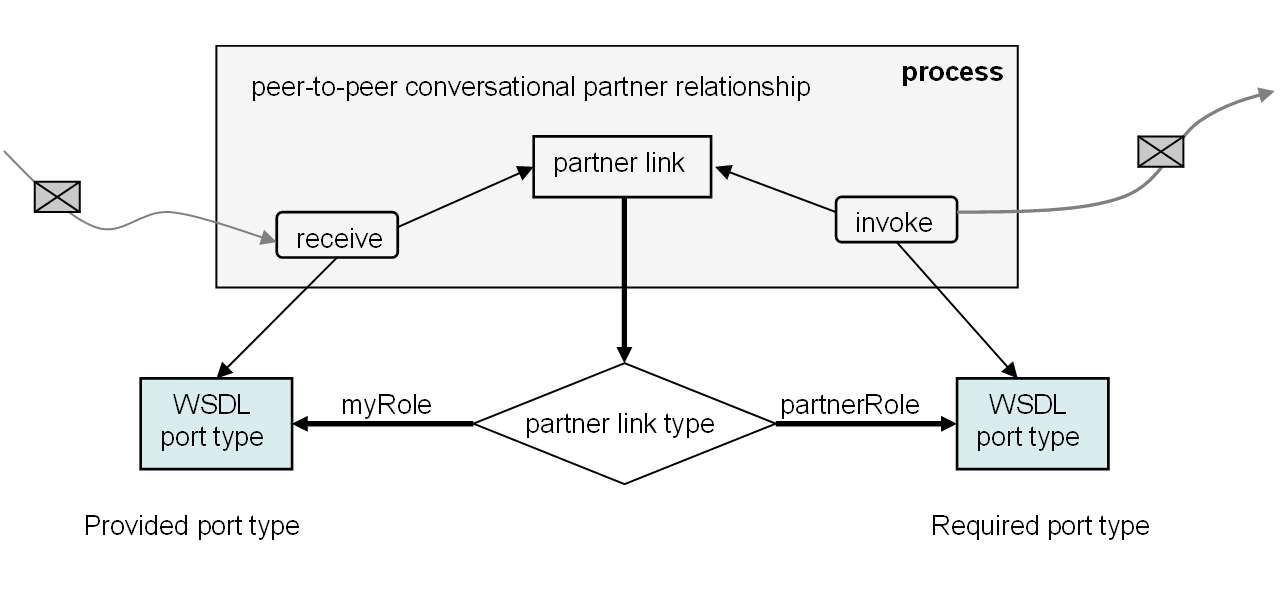
\includegraphics[width=0.82\textwidth]{bilder/partnerLink.png}
		\caption{Partner Link\cite{Dieter}}
	\label{fig:partnerLink}
\end{figure}

\subsection{BPEL Prozess}
BPEL-Prozess ist definiert in Form eines XML-Dokuments. Die Wurzel eines BPEL-Dokuments ist das Element $<$process$>$, welches die Struktur und den
Kontrollfluss eines Gesch�ftsprozesses in sich kapselt. Das Prozess-Element enth�lt drei wichtige Abschnitte:

\begin{itemize}
	\item $<$partnerLinks$>$ - Partner Link-Definitionen, die f�r Kommunikation mit den Partner benutzt werden.   
	\item $<$variables$>$ -  Variablen f�r die Speicherung von internen Daten und Daten, die Empfangen oder Gesendet werden.  Alle in diesem Bereich definierten Variablen sind globale Variablen. Es gibt M�glichkeit lokale Variablen zu definieren. Sie werden in einem Sichtbarkeitsbereich
(Scope) durch einen eindeutigen Namen und einen Datentyp definiert. 
	\item $<$activity$>$ - Gesch�ftslogik in Form von Aktivit�ten. 
\end{itemize}
 
Die Gesch�ftslogik wird in BPEL durch so genannte Aktivit�ten realisiert. Es gibt zwei Arten von Aktivit�ten: Basisaktivit�ten (basic activities) und Strukturierte Aktivit�ten (structured activities). Basisaktivit�ten beschreiben die elementaren Schritte des Prozesses. Strukturierten Aktivit�ten bestimmen den Kontrollfluss und k�nnen deswegen weitere Basis- oder Strukturierten Aktivit�ten enthalten. 

Die Basisaktivit�ten repr�sentieren einzelne Aktionen:
\begin{itemize}
\item $<$invoke$>$ - Aufruf anderer Web Services aus dem Prozess heraus. 
\item $<$receive$>$ - Blockierendes Warten auf Nachrichten.
\item $<$reply$>$ - Versenden einer Antwort.
\item $<$assign$>$ - Zuweisung und Manipulation von Variablenwerten.
\item $<$throw$>$ - Explizites Signalisieren eines Fehlers, welcher durch Fehlerbehandlungen abgefangen werden kann.
\item $<$exit$>$ - Beenden einer Prozessinstanz.
\item $<$wait$>$ - Warten auf einen Zeitpunkt oder f�r eine Zeitspanne.
\item $<$empty$>$ - Nichts machen (NOP).
\item $<$compensate$>$ - Kompensation aller eingebetteten Scopes, $<$compensate$>$ kann nur im FaultHandler
oder CompensationHandler eingebettet sein.
\item $<$compensateScope$>$ - Kompensation
eines speziellen Scope.
\item $<$rethrow$>$ - Wieterreichen der abgefangenen Fehler.
\item $<$validate$>$ - Validierung der Variablenwerten gegen XML-Schema.
	\end{itemize}
Mit den ersten drei lassen sich alle Kommunikationsszenarien implementieren:
\begin{itemize}
	\item synchrone request\slash response-Kommunikation
	\item asynchrone request\slash response-Kommunikation
	\item \textit{one way}-Kommunikation
\end{itemize}

WS-BPEL beschreibt den Ablauf von Gesch�ftsprozessen als strukturierte Aktivit�ten:
\begin{itemize}
\item $<$sequence$>$ - sequentielle Ausf�hrung von Aktivit�ten
\item $<$if$>$ - bedingte Auf�hrung von Aktivit�ten.\textit{ if}-Aktivit�t besitzt mehrere geordnete Bedingte Zweige definiert  durch $<$\textit{if}$>$- und $<$\textit{elseif}$>$- Elemente gefolgt von einem optionalem $<$\textit{else}$>$-Element. Der erste Zweig mit der zutreffenden Bedingung wird ausgef�hrt. 
\item $<$while$>$ - iterative Ausf�hrung der Aktivit�ten. Die Ausf�hrung findet solange statt, bis die Bedingung nicht mehr erf�llt ist. Die Auswertung der Bedingung findet vor jeder Schleifenausf�hrung statt.
\item $<$repeatUntil$>$ - iterative Ausf�hrung von Aktivit�ten. Die Ausf�hrung findet solange statt, bis die Bedingung erf�llt ist. Die Auswertung der Bedingung findet nach jeder Schleifenausf�hrung statt.
\item $<$forEach$>$ -  Ausf�hrung mehrerer Scopes. Die Ausf�hrung kann entweder seriell oder parallel erfolgen (gesteuert durch Attribut \textit{parallel}).
\item $<$pick$>$ - blockierendes Warten auf  Eintreffen eines von mehreren Ereignissen. Bei dieser strukturierenden Aktivit�t wird ein Zweig aus mehreren anhand eines Ereignisses (Nachricht oder Alarm) ausgew�hlt. Wurde ein zutreffendes Ereignis empfangen, so wird die zugeh�rige Aktivit�t ausgef�hrt und alle nachfolgenden Ereignisse verworfen. 
\item $<$flow$>$ - erm�glicht parallele Ausf�hrung von Aktivit�ten mit Synchronisationsm�glichkeit (siehe Abschnitt \ref{sec:linkkonzept}).  
\end{itemize}



\subsection{Link-Konzept}\label{sec:linkkonzept}
 In einer flow-Aktivit�t k�nnen Links definiert werden. Sie dienen
der Synchronisation nebenl�ufiger Aktivit�ten. Jeder Link verbindet eine
\textit{source}-  mit einer \textit{target}-Aktivit�t und besitzt eine implizite oder explizite \textit{transition condition} (boolscher Ausdruck). Ist der Ausdruck nicht spezifiziert, so ist der Wert der \textit{transition condition} \textit{true}. Jede Aktivit�t, die das Ziel eines Links ist, hat eine implizite oder explizite \textit{join condition} (boolscher Ausdruck). Im impiziten Fall ist das eine ODER-Verkn�pfung der Status aller eingehenden Links. Die Auswertung dieser Bedingungen bei der Ausf�hrung wird an einem kleinem Beispiel erl�utert.

\begin{figure}[h!]
	\centering
		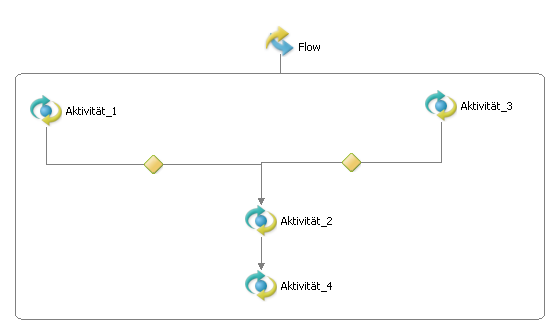
\includegraphics[width=0.53\textwidth]{bilder/FlowBespielLinks.png}
	\caption{Beispiel einer flow-Aktivit�t mit Synchronisationslinks}
	\label{}
\end{figure}

Ist die Ausf�hrung der Aktivit�t \textit{activity\_1} beendet, so wird \textit{transition condition} des Links \textit{link\_1} ausgewertet und der Status auf den entsprechenden Wert \textit{true} oder \textit{false}  gesetzt. Auf dieselbe Weise wird der Status des zweiten Links ermittelt. Stehen die Status der beiden Links fest, so kann die \textit{join condition} der Aktivit�t \textit{activity\_3} ausgewertet werden. Bei einem \textit{true}-Wert wird die Ausf�hrung des Prozesses  ganz normal mit \textit{activity\_3}  fortgesetzt. Ist der Wert \textit{false}, so wird eine Fehlermeldung (\textit{Join Failure}) erzeugt und der Kontrollfluss f�r Fehlerbehandlung aktiviert. Ist dieses Verhalten unerw�nscht, so kann das Standardattribut \textit{suppressJoinFailure} auf den Wert \textit{"`yes"'} gesetzt. In diesem Fall wird \textit{activity\_3} ebenfalls nicht ausgef�hrt, allerdings wird der Prozess ganz normal, ohne eine Fehelermeldung zu produzieren, mit der \textit{activity\_4} fortgesetzt.

Ist \textit{activity\_2} zum Beispiel in einem \textit{if}-Zweig, der w�hrend der Ausf�hrung nicht aktiviert wird, so kann der Status des ausgehenden Links nicht auf die normale Weise ermittelt werden. Die \textit{join condition}  kann ohne des Status des zweiten Links nicht ausgewertet werden.  Das w�rde zu einer Blockierung des Kontrollflusses bei \textit{activity\_3} f�hren. F�r solche Situationen sieht BPEL \textit{Dead-Path-Elimination} vor. Wird eine Aktivit�t aufgrund einer zu
\textit{false} ausgewerteten \textit{join condition}
oder eines nicht abgearbeiteten Zweiges einer if- oder pick-Aktivit�t nicht
ausgef�hrt, so wird f�r alle eventuell vorhandenen ausgehenden Links die \textit{transition condition}
auf \textit{false} gesetzt. Diese Werte werden soweit wie m�glich entlang des Pfades propagiert. Auf die Weise werden Pfade eliminiert, die nicht zur Ausf�hrung kommen, und damit Blockierungen des Kontrollflusses vermieden.

Bei der Verwendung von Links ist folgendes zu beachten:
\begin{itemize}\label{restrictions}
	\item ein Link darf genau eine \textit{source} und eine \textit{target}-Aktivit�t verbinden,
	\item Links d�rfen keine Zyklen bilden,
	\item es m�ssen \textit{boundary crossing}-Restriktionen beachtet werden:
\begin{itemize}
	\item Links d�rfen nicht in oder aus den Wiederholungsschleifen und \textit{Compensation Handler} ein- bzw. austreten
	\item Links d�rfen aus den \textit{Fault} und \textit{Termination Handler} nur austreten
	\item Links, die aus den \textit{catch} oder \textit{catchAll}-Bl�cken des Fault Handlers oder aus dem Termination Handler austreten, m�ssen in einem nicht zu den Handlern zugeh�rigem \textit{Scope} landen.)
\end{itemize}
\end{itemize}

\subsection{\textit{Scope}}
\textit{Scopes} dienen zur Strukturierung von BPEL-Prozessen und definieren Sichtbarkeitsbereiche f�r Variablen und Ereignisse. Ein \textit{Scope} ist ein Ausfuhrungskontext f�r Aktivit�ten mit der M�glichkeit,  eigene Fault, Compensation, Termination und Event Handler zu definieren. Das $<$process$>$-Element ist ein impliziter globaler Scope (Prozess-Scope).
\subsubsection{\textit{Event Handler}}
 BPEL bietet die M�glichkeit, parallel zum normalen Kontrollfluss bestimmte Ereignisse
mit so genannten \textit{Event Handlern} zu behandeln. \textit{Event Handler} geh�ren zu einem
bestimmten \textit{Scope} innerhalb des Prozesses oder zu dem globalen Prozess \textit{Scope}.
Sie behandeln Ereignisse, die den zugeordneten G�ltigkeitsbereich betreffen.
Innerhalb eines \textit{Event Handlers} k�nnen beliebige Abfolgen von BPEL Aktivit�ten definiert
werden. Es gibt zwei Typen von Ereignissen, auf die in einem \textit{Event Handler} reagiert werden kann: Nachrichten und zeit gesteuerten Ereignisse.

\subsubsection{Fehlerbehandlung und Kompensation}
  BPEL-Sprache hat wie viele moderne Programmiersprachen ein Konzept zur strukturierten Behandlung von Laufzeitfehlern.
  Tritt ein Fehler im laufenden Prozess auf, so wird ein f�r diesen Bereich zust�ndiger \textit{Fault Handler} aufgerufen. 
  Oft m�ssen im Fehlerfall bereits abgeschlossene Aktivit�ten kompensiert werden. In BPEL kann
daf�r ein \textit{Compensation Handler} definiert werden, in dem Aktivit�ten f�r die Kompensation festgelegt werden.
\textit{Compensation Handler} k�nnen nur aus \textit{Fault Handler} oder \textit{Compensation Handler} des umschlie�enden \textit{Scopes} aufgerufen werden. Au�erdem ein \textit{Compensation Handler} kann nur f�r \textit{Scopes} aufgerufen werden, die
ordnungsgem�� abgearbeitet wurden. Jedes \textit{Scope} besitz ein Fault und \textit{Compensation Handler}, der Prozess selbst hat in BPEL 2.0 nur den \textit{Fault Handler}. 
  
Ist kein benutzerdefiniertes \textit{Fault Handler} spezifiziert, so gibt es ein impliziter \textit{Fault Handler}, der die \textit{Compensation Handler}
aller direkt eingeschlossener \textit{Scopes} in der umgekehrten Reihenfolge ihrer Abarbeitung aufruft und
anschlie�end den Fehler an den umschlie�enden Scope oder den Prozess selbst weiter reicht. Es k�nnen eigene \textit{Fault Handler} spezifiziert werden, der
je nach Art des auftretenden Fehlers eine bestimmte BPEL-Aktivit�t ausf�hrt. F�r die Bindung bestimmter Aktivit�ten an die bestimmten Fehler werden \textit{catch} und \textit{catchAll}-Elemente verwendet.
  
Die Fehler k�nnen auch in den \textit{Compensation} und in den \textit{Fault Handler} selbst auftreten. In die Abbildung \ref{fig:ScopeFaultCompensation2} wird der Zusammenhang zwischen \textit{Handler} und \textit{Scopes} grafisch dargestellt. Die Pfeile zeigen dabei den m�glichen Kontrollfluss. 
\begin{figure}[h!]
	\centering
		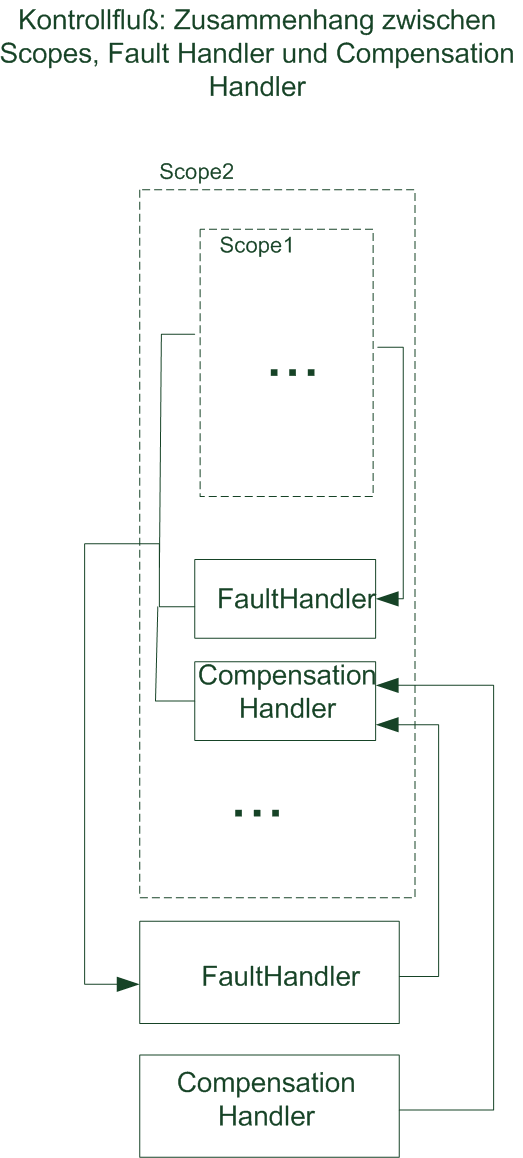
\includegraphics[width=0.33\textwidth]{bilder/ScopeFaultCompensation2.png}
	\caption{Zusammenhang zwischen Scopes, Fault und Compensation Handler}
	\label{fig:ScopeFaultCompensation2}
\end{figure}

 Als einzige Ausnahme bietet \textit{invoke}-Aktivit�t die M�glichkeit, eigene \textit{Fault} und \textit{Compensation Handler} zu definieren. Es entspricht einem expliziten \textit{Scope}, das die \textit{invoke}-Aktivit�t umschlie�t und \textit{Compensation} und \textit{Fault Handler} besitzt.

\subsubsection{Termination Handler}
Scopes besitzen die M�glichkeit, auf den Ablauf einer erzwungenen Terminierung Einfluss zu
nehmen. Das Verhalten wird innerhalb eines Termination Handler festgelegt, der im Falle einer erzwungenen Terminierung nach der
Beendigung aller laufenden Aktivit�ten des Scope ausgef�hrt wird. Ist kein
Termination Handler definiert, wird ein Standard-Termination-Handler aktiviert. Dieser kompensiert
alle erfolgreich beendeten eingebetteten Scopes in der umgekehrten Ausf�hrungsreihenfolge. Er verh�lt sich also wie der Standard-Fault-Handler.

\subsection{Prozessinstance}
Die Erzeugung von Prozessinstanzen erfolgt implizit anhand von Aktivit�ten (\textit{receive} oder \textit{pick}),
beim Eintreffen von externen Nachrichten. Die entsprechenden Aktivit�ten werden mit dem Attribut \textit{createInstance}=\textit{"'yes"'} gekennzeichnet.  
Zur
Identifikation von laufenden Prozessinstanzen dienen so genannten \textit{Correlation Sets}. Diese werden von BPEL-Engine verwendet, um Nachrichten an richtige Instanzen weiterleiten zu k�nnen.

Prozessinstanzen werden beendet, wenn die Aktivit�ten, die das Verhalten von Prozessen bestimmen,
abgearbeitet wurden (normale Beendigung), wenn ein Fehler den Prozess-\textit{Scope} erreicht,
der entweder behandelt oder nicht behandelt wird, oder wenn von Prozessinstanzen die \textit{exit}-
Aktivit�t ausgef�hrt wurde.


   

\subsection{Engine}
Ein BPEL-Prozess besteht aus der Gesch�ftslogik (definiert in BPEL), Servicebeschreibung (WSDL) und optional aus weiteren Datentypen (XML Schema). Diese Informationen werden zusammengefasst und in eine BPEL Engine deployt. Die Engine ist unter anderem daf�r verantwortlich, die \textit{Endpoints} der Partner des BPEL Prozesses zu spezifizieren. F�r jeden Link muss bekannt sein, welche WSDL-service und -port und welche Adresse f�r die Kommunikation benutzt werden sollen. Diese Information wird in so genannten \textit{Deployment Descriptoren} festgelegt.

\textbf{ActiveBPEL Engine}.
Die ActiveBPEL-Engine ist eine Runtime-Umgebung f�r die Business Process Execution Language, die in Java implementiert und sowohl BPEL 1.1 als auch BPEL2.0 konform ist. 
Die Engine l�uft innerhalb des Apache Tomcat Servers und stellt dort die zum automatischen Gesch�ftsprozess zusammengefassten Web Services - wiederum als Web Service - zur Verf�gung. Zum Deployen wird eine Archivdatei, die das BPEL-Modell, WSDLDateien
und den Engine-spezifischen Deployment Descriptor enth�lt, in das bpr-Verzeichnis
des Servers, auf dem die ActiveBPEL-Engine l�uft, abgelegt. 

\subsection{BPEL Prozess}

Die Business Process Execution Language for Web Services (BPEL4WS) ist eine XML-
basierte Sprache zur Beschreibung der Aggregation vonWeb Services. Sie entstand durch die
Vereinigung der Sprachen WSFL von IBM [Ley01] und XLANG von Microsoft [Tha01]. Ge-
schuldet ihrer Entstehungsgeschichte besitzt die Sprache BPEL4WS eine beachtliche Kom-
plexit�at teilweise mit redundanten sowie mehrdeutig beschriebenen Konzepten. Au�erdem
wurden die Wechselwirkungen der verschiedenen Konzepte im Vorhinein nicht ausreichend
untersucht. Aus diesem Grund ist die De�nition einer formalen Semantik f�ur BPEL4WS ei-
nes der grundlegenden Ziele in diesem Forschungsprojekt. Um die praktische Relevanz sicher
zu stellen, formulieren wir eine Reihe von Anforderungen an die entstehenden Semantik:


In diesem Abschnitt stellen wir sehr grob die grundlegenden Konzepte der Sprache
BPEL4WS vor. In der weiteren Arbeit werden die einzelnen Konzepte anhand von Bei-
spielen genauer erl�autert. Dar�uber hinaus bieten die Spezi�kation der Sprache [ACD+02]
und Tutorials auf der Web-Seite von IBM [Tid00] tiefer gehende Informationen.
Ein Modell der Sprache BPEL4WS beschreibt die interne Struktur eines Web Service und
dessen Einbindung in die Umwelt, d. h. ein Modell besteht aus einer Menge von Aktivit�aten
die zu einem Prozess zusammengefasst werden und einer Menge von Nachrichtenkan�alen
(Operationen von Porttypen), die Partnern angeboten oder von diesen verlangt werden.
Wir beginnen zuerst mit der internen Struktur:
Aktivit�aten
Im Zentrum der Modellierung von Gesch�aftsprozessen stehen die Aktivit�aten und ihre kau-
salen Zusammenh�ange. In BPEL4WS gibt es zwei Sorten von Aktivit�aten: Basic Activities
und Structured Activities.
Die einfachen Aktivit�aten repr�asentieren atomare Einheiten und lassen sich erneut in
zwei Gruppen teilen: F�ur die Kommunikation mit einem anderen Web Service sind die
Aktivit�aten invoke, receive und reply zust�andig. Mit invoke kann ein anderer Web Service
aufgerufen werden, d. h. es wird eine Nachricht an diesen gesendet und gleich oder sp�ater
eine Antwort erwartet. Mit receive wird ein Aufruf (eine Nachricht) von einem anderen Web
Service entgegen genommen und mit reply dieser beantwortet.
Die zweite Gruppe der einfachen Aktivit�aten repr�asentieren interne Schritte: assign ist
eine Wertzuweisung, wait ist ein Timer und empty ist eine leere Aktivit�at. Teilweise steuern
sie auch den weiteren Prozessverlauf: terminate bricht den Prozess ab, throw wirft einen
Fehler und compensate veranlasst die R�ucksetzung eines Teils des Prozesses.
Neben den einfachen Aktivit�aten gibt es in BPEL4WS auch f�unf Klassen strukturierter
Aktivit�aten. Mit diesen Aktivit�aten wird der Kontroll�uss abgebildet: Die einfachste ist se-
quence, diese Aktivit�at de�niert die sequentielle Ordnung einer Menge anderer Aktivit�aten.
Die alternative Auswahl zwischen Aktivit�aten ist mit Hilfe von pick und switch m�oglich, bei
pick entscheidet eine Nachricht von au�en, bei switch wird durch die Auswertung von Daten
eine Entscheidung getro�en. Mit der Aktivit�at while ist es m�oglich, zyklisches Verhalten
zu de�nieren. Letztlich dient die Aktivit�at �ow dazu, eine unabh�angige Menge von Akti-
vit�aten zu spezi�zieren. Innerhalb von �ow k�onnen die Aktivit�aten durch zus�atzliche links
untereinander synchronisiert werden. Jede der strukturierten Aktivit�aten enth�alt ihrerseits
mindestens eine Aktivit�at. Auf diese Weise k�onnen durch Schachtelung beliebig komplexe
Kontroll�uss-Beziehungen gebildet werden.
Ein Sonderrolle spielt die Aktivit�at scope.
�U
b
e
r
w
a
c
h
t
e
A
k
t
i
v
i
t
�a
t
e
n
In BPEL4WS ist es m�oglich, eine einzelne Aktivit�at unter besondere Beobachtung zu stel-
len, d. h. auftretende Fehler abzufangen, auf externe Ereignisse zu reagieren und ggf. die
Aktivit�at nach erfolgreicher Ausf�uhrung zu kompensieren, wenn es die �au�eren Umst�an-
de verlangen. Zu diesem Zweck gibt es das Konzept des scopes als Aggregation aus event
handler, fault handler, compensation handler und einer �uberwachten Aktivit�at. Auf der
einen Seite kann die �uberwachte Aktivit�at wiederum strukturiert sein, so dass der scope
eine Menge von Aktivit�aten �uberwachen kann. Auf anderen Seite kann der scope selbst als
eine Aktivit�at aufgefasst werden und damit in einer strukturierten Aktivit�at vorkommen.
Prozesse
Aktivit�aten k�onnen ineinander geschachtelt sein und bilden somit eine hierarchische Struk-
tur { einen Aktivit�aten-Baum. DieWurzel dieses Baumes ist der Prozess: Ein Prozess besitzt
genau eine Aktivit�at. Neben dieser Aktivit�at kann ein Prozess event handler, fault handler
und compensation handler besitzen, d. h. ein Prozess ist auch gleichzeitig ein scope.
In BPEL4WS geh�ort zu einem Web Service genau ein Prozess. Es ist m�oglich, diesen Pro-
zess pr�azise und vollst�andig zu modellieren. Auf diese Weise gelangt man zu einem direkt
ausf�uhrbaren Prozessmodell (= Executable Process). Dar�uber hinaus gestattet BPEL4WS
eine abstrakte Spezi�kation des Verhaltens (= Business Protocol). Die abstrakte Spezi-
�kation ist ein wesentlicher Teil der ver�o�entlichten Beschreibung des Web Service. Ein
potentieller Anwender entscheidet aufgrund dieser Spezi�kation, ob der vorliegende Web
Service mit seiner Komponente kompatibel ist. Im Rahmen dieser Arbeit werden wir die
Kompatibilit�at zweier Web Services de�nieren (siehe Abschnitt 3.1.4).
Die De�nition der Kommunikation innerhalb des Prozesses st�utzt sich auf die De�nition
der Schnittstelle des Web Service mit WSDL ab.
Kommunikation
Ein Web Service ist ein o�enes System, dass mit anderen Komponenten (o. B. d. A. eben-
falls Web Services) �uber Nachrichtenaustausch kommuniziert. Jede Nachricht ist ein XML-
Dokument, wobei die Typ der Dokumente bereits im WSDL-Modell des Web Service de�-
niert werden. Als konsequente Weiterf�uhrung verwendet BPEL4WS f�ur interne Datenstruk-
turen (variables) ebenfalls XML-Dokumente.
Die Schnittstelle f�ur die Kommunikation wird in WSDL de�niert: Eine Nachrichten ist
ein XML-Dokument, das Senden und empfangen einer Nachricht (mit oder ohne Feedback)hei�t Operation. Eine Menge von Operationen wird zu einem Porttype zusammengefasst.
Jeder Web Service bietet eine Menge von Porttypen an.
Die Kommunikation �uber einen Porttypen kann man von zwei Seiten aus betrachten:
Auf der einen Seite gibt es den Web Service, der diesen Porttypen anbietet und auf der
anderen Seite gibt es einen Web Service, der diesen Porttypen von au�en benutzt. Deshalb
wird in BPEL4WS die Verbindung zwischen den Operationen eines Porttypen und den
Aktivit�aten im Prozess durch PartnerLinks abgebildet: Die Aktivit�at receive und reply
implementieren eine Operation an der Schnittstelle dieses Web Service und stellen damit
einem anderem Web Service Funktionalit�at zur Verf�ugung, die Aktivit�at invoke spezi�ziert
eine Operation an der Schnittstelle eines anderen Web Service und benutzt damit dessen
Funktionalit�at. Da ein anderer Web Service (d. h. ein Partner) in einem BPEL4WS-Modell
sowohl Funktionalit�at anbieten als auch benutzen kann, wird ein Partner durch eine Menge
von PartnerLinks spezi�ziert.


BPEL4WS (kurz BPEL) unterscheidet zwischen ausf�hrbaren und abstrakten Prozessen, wobei
die Unterscheidung f�r diese Arbeit irrelevant ist. Ein BPEL4WS Prozess selbst kann als
ein Ablaufdiagramm angesehen werden, wobei jeder Knoten eine Aktivit�t darstellt. Hierbei
wird zwischen primitiven und strukturierten Aktivit�ten unterschieden. Die primitiven Aktivit�ten
erm�glichen es: Operationen auf anderen Web Services aufzurufen (invoke), auf
Nachrichten von externen Partnern zu warten (receive), Antworten auf eine Anfrage zu verschicken
(reply), eine bestimmte Zeit zu warten (wait), den Variablen Werte zuzuweisen
(assign), Fehler zu generieren (throw), den gesamten Service explizit zu beenden (terminate)
oder auch nichts zu tun (empty). Die strukturierten Aktivit�ten erm�glichen es die
primitiven zu einer komplexeren Einheit zu kombinieren. Es ist m�glich, folgendes mit strukturierten
Aktivit�ten zu realisieren: Eine geordnete Sequenz der Aktivit�ten zu definieren
(sequence), Verzweigungen innerhalb eines Prozesses zu bilden (switch), Schleifen zu
definieren (while), Entscheidungen nach Ablauf bestimmter Zeit oder anhand externer
Trigger zu treffen (pick) und Aktivit�ten parallel auszuf�hren (flow). Au�erdem k�nnen
mit Hilfe des control links Konstrukts Ausf�hrabh�ngigkeiten zwischen parallelen Aktivit�ten
definiert werden.
BPEL basiert auf mehreren XML-Spezifikationen: WSDL 1.1 [W3C (2001)], XML Schema
1.0 [W3C (2000)], XPath 1.0 [W3C (1999)] und WS-Addressing [Microsoft et al. (2003b)].
WSDL und XML Schema Typdefinitionen bieten das Datenmodell, das bei BPEL4WS Pro zessen genutzt wird, an. XPath liefert die Unterst�tzung f�r Datenmanipulation. Alle externen
Ressourcen und Partner werden als WSDL Services repr�sentiert. BPEL ist leicht anpassbar,
so dass neue Versionen von den oben genannten Standards leicht �bernommen werden
k�nnen. Mehr �ber die Integration der XML-Standards in BPEL4WS ist in der Spezifikation
[Microsoft et al. (2003a)] zu finden.
Wie oben bereits erw�hnt ist der Hauptzweck von BPEL4WS Prozessen Web Services zu
kombinieren und zu koordinieren, wichtig ist aber auch dass ein BPEL4WS Prozess selbst als
ein Web Service nach au�en wirken kann.
Die Arbeit bezieht sich auf die Version 1.0 von BPEL4WS, die im August 2002 erschienen
ist. Die Abgrenzung zur aktuellen Version 1.1 ist im Kapitel 5 zu finden

zessen genutzt wird, an. XPath liefert die Unterst�tzung f�r Datenmanipulation. Alle externen
Ressourcen und Partner werden als WSDL Services repr�sentiert. BPEL ist leicht anpassbar,
so dass neue Versionen von den oben genannten Standards leicht �bernommen werden
k�nnen. Mehr �ber die Integration der XML-Standards in BPEL4WS ist in der Spezifikation
[Microsoft et al. (2003a)] zu finden.
Wie oben bereits erw�hnt ist der Hauptzweck von BPEL4WS Prozessen Web Services zu
kombinieren und zu koordinieren, wichtig ist aber auch dass ein BPEL4WS Prozess selbst als
ein Web Service nach au�en wirken kann.
Die Arbeit bezieht sich auf die Version 1.0 von BPEL4WS, die im August 2002 erschienen
ist. Die Abgrenzung zur aktuellen Version 1.1 ist im Kapitel 5 zu finden
zessen genutzt wird, an. XPath liefert die Unterst�tzung f�r Datenmanipulation. Alle externen
Ressourcen und Partner werden als WSDL Services repr�sentiert. BPEL ist leicht anpassbar,
so dass neue Versionen von den oben genannten Standards leicht �bernommen werden
k�nnen. Mehr �ber die Integration der XML-Standards in BPEL4WS ist in der Spezifikation
[Microsoft et al. (2003a)] zu finden.
Wie oben bereits erw�hnt ist der Hauptzweck von BPEL4WS Prozessen Web Services zu
kombinieren und zu koordinieren, wichtig ist aber auch dass ein BPEL4WS Prozess selbst als
ein Web Service nach au�en wirken kann.
Die Arbeit bezieht sich auf die Version 1.0 von BPEL4WS, die im August 2002 erschienen
ist. Die Abgrenzung zur aktuellen Version 1.1 ist im Kapitel 5 zu finden zessen genutzt wird, an. XPath liefert die Unterst�tzung f�r Datenmanipulation. Alle externen
Ressourcen und Partner werden als WSDL Services repr�sentiert. BPEL ist leicht anpassbar,
so dass neue Versionen von den oben genannten Standards leicht �bernommen werden
k�nnen. Mehr �ber die Integration der XML-Standards in BPEL4WS ist in der Spezifikation
[Microsoft et al. (2003a)] zu finden.
Wie oben bereits erw�hnt ist der Hauptzweck von BPEL4WS Prozessen Web Services zu
kombinieren und zu koordinieren, wichtig ist aber auch dass ein BPEL4WS Prozess selbst als
ein Web Service nach au�en wirken kann.
Die Arbeit bezieht sich auf die Version 1.0 von BPEL4WS, die im August 2002 erschienen
ist. Die Abgrenzung zur aktuellen Version 1.1 ist im Kapitel 5 zu finden

BPEL ist eine XML-basierte Sprache f�r die Definition
und Ausf�hrung von Gesch�ftsprozessen unter
Verwendung von Web Services
 BPEL integriert individuelle Web Services zu
Gesch�ftsprozessen.
 Jeder BPEL Prozess ist ein ausf�hrbares und portables
Script
 BPEL erm�glicht die Realisierung service-orientierter
Architekturen durch Komposition, Orchestrierung und
Koordination von Web Services.
 BPEL ist plattform- und anbieterunabh�ngig
 ausgedr�ckt in XML
 verwendet und erweitert WSDL
 verwendet WSDL und XML Schema f�r Datenmodelle

Ein Gesch�ftsprozess und ein Web Service sind in gewissem Sinn das
gleiche. Wenn man einen Web Service aufruft, weiss man nicht, ob es
sich um einen atomaren Service handelt oder um einen komplexen,
aus mehreren Services bestehenden Prozess.

BPEL spezifiziert das Verhalten von Gesch�ftsprozessen
durch Web Services und als Web Service:
Jeder BPEL Prozess ist auch ein Web Service

Web Services k�nnen auf zwei Arten kombiniert werden:
Orchestration: Ein zentraler Prozess koordiniert die
Operationen der Web Services, die in den Prozess
eingebunden sind.
Choreography: Es gibt keinen zentralen Koordinator. Jeder in
die Choreography eingebunden Web Service "weiss", mit
wem er zu interagieren hat. Bei der Choreographie erfolgt
die Zusammenarbeit �ber den Austausch von Nachrichten
in einem �ffentlichen Prozess.

BPEL unterst�tzt Orchestration und Choreography durch
Executable Processes: Spezifikation eines
Gesch�ftsprozesses, der durch eine Orchestration Engine
ausgef�hrt wird
Abstract Business Protocols: Spezifikation des
Nachrichtenaustauschs zwischen Partnern folgt dem
Choreographie Paradigma

Setzt auf XML und Web Services auf
Verbindung von 2 fr�heren Workflow-Sprachen:
WSFL: Web Services FlowLanguagevon IBM
Konzept: gerichtete Graphen, Aktivit�ten mit Kontroll-und Datenfl�ssen verbunden
XLANG: Web Services forBusiness ProcessDesign von Microsoft
Konzept: Flussdiagramm mit einfachen Kontrollstrukturen wie Sequence, Switch, While, All (parallele Ausf�hrung)
Erweiterung der WSDL-Service-Beschreibung

Business ProcessExecutionLanguage:
XML-basierte Prozessbeschreibungssprache, aktuell Version 2.0
Abbildung von Gesch�ftsprozessen auf Basis von Web Services
BPEL-Prozess wird durch Interaktion der WSDL-portTypesrealisiert
Aktivit�t = ein Prozessschritt innerhalb des Gesamtprozesses
WSDL-Datei beschreibt Sicht von au�en
Beschreibung m�glicher Rollen
Port mit aufrufbaren Operationen
BPEL-Datei beschreibt Ablauf des Gesch�ftsprozesses
Reihenfolge der Aktivit�ten
Randbedingungen
Fehlerbehandlungen


WSDL-Messagesdefinieren
Verwendete Nachrichten
WSDL-PortTypesdefinieren
Verf�gbare Schnittstellen zu Diensten
PartnerLinkTypesdefinieren
Rollen der PortTypes
PartnerLinksdefinieren
verkn�pfen WSDL-portTypesmit BPEL-Prozess-Definitionen
Verwendete Variablen definieren
Eigentlichen Prozess definieren

Variablen m�ssen vor Verwendung deklariert werden
M�gliche Datentypen:
WSDL messagetype
XML Schema simple type
XML Schema element


Vorteil
Unterst�tzung vieler verschiedener Anbieter
Erm�glicht Prozessinteroperabilit�t
XML-basiert
Umfangreiche Kontrollfluss-Beschreibung, vielseitige Verschachtelung
Basiert auf vorhandenen WS-/XML-Standards, z.B. BPEL 1.1 auf WSDL 1.1, XML Schema 1.0, XPath1.0 und WS-Addressing
Synchrone und asynchrone Nachrichten�bermittlung
Callbacksund CorrelationSets f�r Komposition
Unterst�tzung f�r Transaktionen (atomar und lang-andauernd)
Ausnahmebehandlung, Kompensationen und Fehlerbehandlung

Prtener Link ist ein Kommunikationskanal 
Process-Element:
\begin{itemize}
	\item Partner link
	\item variables section
	\item activity
\end{itemize}
 
\subsection{Gesch�ftslogik mit BPEL}
Aktivit�ten sind Statements des BPEL-Programms



\subsubsection{Basisaktivit�ten}

\begin{itemize}
	\item receive
	\item invoke
	\item reply
	\item wait
	\item empty
	\item terminate
\end{itemize}
Mit den ersten drei lassen sich alle Kommunikationsszenarien implementieren.
\subsubsection{Strukturierte Aktivit�ten}
Strukturierte Aktivit�ten bestimmen die Reihenfolge in der die eingeschlo�ene Aktivit�ten ausgef�hrt werden. K�nnen geschachtelt werden.

\begin{itemize}
	\item secuence 
	\item switch 
	\item while
	\item flow
	\item pick
\end{itemize}

Die ersten drei entsprechen den konventionellen strukturierten Programmierung
\subsubsection{Fault handling und compensation}
    Kontrollfluss bei Asnahmenbehandlung
\subsubsection{Processinstance und Lifecycle}
\subsection{BPEL Ausf�hrungsumgebung}
\section{BPEL Testen}
  

\subsection{BPELUnit Framework}
\subsubsection{Konzepte}
\subsubsection{Spezifikation, Organisation und Ausf�hrung der Tests}
\subsubsection{Clients}
\section{Abdeckung, als Ma� f�r die Testqualit�t}
Um die Softwarequalit�t anhand der Test bewerten zu k�nnen, m�ssen zus�tzliche
Informationen �ber die Tests bekannt sein. Wichtig sind unter anderem die Anforderungs-,
Code- und Datenabdeckung der Tests.
\begin{itemize}
	\item \textbf{Anforderungsabdeckungsmetriken} (\textit{eng. requirements coverage}) ist eine funktionale
Abdeckung auf Basis einer Spezifikation, die angibt, inwieweit die Testf�lle alle Anforderungen abdecken. Diese Metrik wird meist im Zusammenhang mit \textit{Black-Box-Tests} verwendet. 
	\item \textbf{Codeabdeckungsmetriken} (\textit{eng. code coverage}) ist eine Metrik f�r das Verh�ltnis zwischen
zu testenden und tats�chlich getesteten Elementen des Pr�flings. Die Tests, die auf der Codeabdeckung basieren, geh�ren zur Gruppe der strukturorientierten Testtechniken und zielen darauf ab, die innere Struktur der Software zu testen (\textit{White-Box-Test}).\cite{MyersJune2004}
\item \textbf{Datenabdeckungsmetriken} (\textit{eng.data coverage})  ist die Metrik, die angibt, wie und wann und in welcher Weise die Variablen verwendet werden (\textit{White-Box-Test}).
\end{itemize}
Die Anforderungs-, Code- und Datenabdeckung sind Mittel zur Messung der Qualit�t bzw. Voll"-st�n"-dig"-keit der Tests. Die beiden Testarten (\textit{Black-Box} und \textit{White-Box}) erg�nzen sich gegenseitig und werden in der Regel kombiniert angewendet. 

Die Aufgabe der BPEL ist, die Web Services in einer bestimmten Reihenfolge zu einer Anwendung zu verkn�pfen. Die Ablauf\-logik, die somit in einer BPEL-Datei gekapselt ist, kann am Besten mit kontrollflussorientierten Tests �berpr�ft werden. F�r die Bewertung solcher Tests eignen sich die Codeabdeckungsmetriken, die damit im Fokus dieser Arbeit stehen. Im weiteren Verlauf dieser Arbeit werden Anforderungs- und Datenabdeckung nicht weiter behandelt. Der Begriff \textit{Testabdeckung} wird ausschlie�lich als Synonym zu Codeabdeckung verwendet. 

Die Unit-Tests werden verwendet, um sicherzustellen, dass der erstellte Code korrekt funktioniert. Jedoch lassen sich dabei nur Aussagen �ber die Codebereiche machen, die im Test aufgerufen oder, anders gesagt, durch den Test abgedeckt wurden. Das zugrundeliegende Prinzip lautet: ist der Code abgedeckt, so ist die Wahrscheinlichkeit h�her, dass es keinen Fehler gibt. Das Ausf�hren aller potentiell fehlerhaften Stellen des Programms ist ein notwendiges Kriterium f�r das Finden der Fehler im Code. Deswegen ist die Angabe der erreichten Codeabdeckung aus der Sicht der Qualit�tssicherung nicht nur sinnvoll, sondern unabdingbar.

Bei der Analyse der Codeabdeckung geht es also darum festzustellen, wie gut die Codebereiche durch die Tests abgedeckt sind bzw. welche Bereiche gar nicht oder nicht ausreichend abgedeckt sind. Wenn ein Testentwickler auf diese Information st�ndig und einfach zugreifen kann, dann hat er die M�glichkeit, neue Tests gezielt zu erstellen. Dadurch kann die Qualit�t der Tests schrittweise erh�ht und die Erstellung �berfl�ssiger Tests vermieden werden. Mit Hilfe der Codeabdeckung kann also ein Optimum zwischen dem wirtschaftlichen Aufwand und der Testqualit�t gefunden werden, was bei der Herstellung der Software auch ein wichtiger Aspekt ist. 

In der folgenden Aussage werden die drei Begriffe \textit{Codeabdeckungsanalyse}, \textit{Testqualit�t} und \textit{Systemqualit�t} in eine Relation zueinander gestellt:
\begin{quotation}
	\textit{W�hrend Unit-Tests dazu dienen, die korrekte
	Funktionsweise der erstellten Software zu verifizieren und die Qualit�t des Gesamtsystems zu steigern, dient die Analyse der Codeabdeckung dazu, die Qualit�t der Tests sicherzustellen und zu erh�hen \cite{Wang2006}}.
\end{quotation}
Demzufolge h�ngt die Codeabdeckung unmittelbar mit der Qualit�t der Tests und indirekten mit der Qualit�t des Gesamtsystems.

 Die bekanntesten Abdeckungsmetriken werden im n�chsten Abschnitt beschrieben.
\subsection{Abdeckungsmetriken }\label{Abdeckungsmetriken}
Es gibt eine Vielzahl von unterschiedlichsten Abdeckungsmetriken. Eine gute �bersicht wird in \cite{Kaner1995} und 
\cite{Zhu1997} gegeben. In diesem Abschnitt werden nur die wichtigsten Abdeckungsmetriken vorgestellt, die f�r diese Arbeit relevant sind.

Als \textit{Testabdeckung} wird �blicherweise das Verh�ltnis zwischen
zu testenden und tats�chlich getesteten Elementen des Pr�flings bezeichnet. Es muss nicht immer 100\% gefordert werden. Je nach festgelegtem Ziel kann auch ein gewisser Anteil festgelegt werden. Die bekanntesten Kriterien sind 
Anweisungs-, Zweig-, Bedingungs- und Pfadabdeckung. In den n�chsten Abschnitten werden die Anweisungs- und Zweigabdeckung vorgestellt. Weitere Metriken werden aufgrund der exponentiell steigenden Anzahl der Testf�lle, die f�r die geforderte Abdeckung notwendig sind, oder geringen Praxisrelevanz nicht behandelt. F�r weitere Informationen zu diesen Metriken wird auf \ref{Liggesmeyer2002} verwiesen. 
\subsubsection{Anweisungsabdeckung}
Die Anweisungsabdeckung (\textit{eng. statement coverage}) ist die einfachste kontrollflussorientierte Metrik.  
Sie wird wie folgt definiert: 
\[
	Anweisungsabdeckung=\frac{\text{\textit{Anzahl der ausgef�hrten Anweisungen}}}{\text{\textit{Anzahl der Anweisungen}}}
\]
Das Ziel der Anweisungsabdeckung ist die mindestens einmalige Ausf�hrung aller Anweisungen des zu testenden Programms.
Bezogen auf den Kontrollflussgraph hei�t es, dass alle Knoten abgedeckt werden m�ssen. Es ist m�glich, mehrerer Anweisungen (z.B. Anweisungen innerhalb einer Schleife) zu einer Einheit
zusammenzufassen, die keinerlei Verzweigungen im Sinne von \textit{if-else}-Anweisungen enth�lt. Wenn die 100\% Anweisungsabdeckung nicht erreicht werden kann, dann ist das ein Hinweis auf den Programmcode, der m�glicherweise unter keinen Umst�nden ausgef�hrt werden kann. 

Anweisungsabdeckung ist ein schwaches Kriterium. Die Fehleridentifizierungsquote ist sehr niedrig. Der Grund daf�r ist, dass die Anweisungsabdeckung nur die einzelnen Anweisungen betrachtet, ohne Zusammenh�nge zu ber�cksichtigen.
\subsubsection{Zweigabdeckung}\label{Zweigabdeckung}
Zweigabdeckung (\textit{eng. branch coverage}) gilt als minimales Kriterium f�r kontrollflussorientierte Testtechniken.
\[
Zweigabdeckung=\frac{\text{\textit{Anzahl der durchlaufenen Zweige}}}{\text{\textit{Anzahl aller Zweige}}}
\]
Das hei�t, dass die hundertprozentige Zweigabdeckung dann erreicht ist, wenn alle Kanten des Kontrollflussgraphen mindestens einmal durchlaufen wurden. Erf�llte Zweigabdeckung stellt sicher, dass alle Verzweigungen des zu testenden Moduls tats�chlich erreichbar sind. Weil das Durchlaufen aller Zweige die Ausf�hrung aller Anweisungen verursacht, impliziert die Zweig\-ab\-deckung die Erf�llung der Anweisungsabdeckung. Mit der Zweigabdeckung k�nnen die nichtausf�hrbaren Programmzweige zus�tzlich aufgesp�rt werden. 

Obwohl die Fehlererkennungsquote gegen�ber der Anweisungsabdeckung steigt, werden nicht alle Aspekte des Kontrollflusses erfasst. Bei den Schleifen wird nur ermittelt, ob diese durchlaufen werden k�nnen.
Obwohl bei der vollst�ndigen Zweigabdeckung jede Entscheidung (komplexe Bedingungen), die Verzweigungen im Kontrollfluss ausl�sen, insgesamt die Wahrheitswerte $true$ und $false$ mindestens einmal annehmen muss, bleiben die Werte der einzelnen Bedingungen unber�cksichtigt. Au�erdem wird jeder Zweig f�r sich alleine betrachtet, ohne die Kombinationen von Zweigen zu ber�cksichtigen. \\[0.5cm]

Eine hohe Testabdeckung bedeutet nicht automatisch, dass der abgedeckte Code optimal getestet wurde. Au�erdem reicht das Erreichen von Abdeckungsvorgaben alleine nicht aus, um die Qualit�t der Software zu garantieren.  Die Testabdeckung ist nur ein Aspekt der Softwareentwicklung, der beim richtigen Einsatz zur Qualit�t der Software beitragen kann.

\nocite{Liggesmeyer2002}
\nocite{Winkler2003}
\chapter{Testabdeckung in BPEL}
Durch die Berechnung der Testabdeckung will der Tester erfahren, wieviel von dem Pr�fling beim Testen ausgef�hrt wurde. F�r die Definition des Pr�flings, in diesem Fall BPEL-Prozesses, wird die BPEL Formalisierung von Ouyang in ??? verwendet. Nach der Pr�sentation der wichtigsten Punkten dieser Formalisierung folgen die Definition der  Aktivit�t- und Zweigabdeckung. Dar�ber hinaus werden zwei spezial f�r BPEL definierten Metriken vorgestellt: Link- und Handlerabdeckung.  
\section{Formale Definition von BPEL}
Die hier vorgestellte formale Beschreibung von WS-BPEL Process Model ist nicht
vollst�ndig und fasst nicht den gesamten Umfang von WS-BPEL um. Es werden nur
f�r diese Arbeit relevante Teile des Modells beschrieben. Als Grundlage dient
eine Definition aus  \cite{Chun2005}, die abgesehen von der Anpassung an den
Standard WS-BPEL 2.0 und einigen Erweiterungen, unver�ndert �bernommen wurde.  

\begin{Def}[WS-BPEL Process Model~\cite{Chun2005}] Ein BPEL-Prozessmodell ist ein Tupel $\mathcal{W=(A,\ E,\ C,\ L,\ HR,\ }type_{\mathcal{A}},\ type_{\mathcal{E}},\
instance,\ name,\ <_{seq},\ <_{if},\\ serialscp,\ process,\ trigger,\ scp_c,\
trigger_c,\ scp_t,\ trigger_{tf},\ \mathcal{LR},\ joincon,\\ 
transitionCondition,\ supjoinf,\ trigger_{jf})$ where: 
\end{Def}
\begin{itemize}
  \item $\mathcal{A}$ ist eine Menge von Aktivit�ten,
  \item $\mathcal{E}$ ist eine Menge von Ereignissen,
  \item $\mathcal{C}$ ist eine Menge von Bedingungen,
  \item $\mathcal{L}$ ist eine Menge von Links (innerhalb von Flow-Aktivit�ten),
  \item sei $\mathcal{B=E\cup C} \cup\{\bot\} $ eine Menge von Marken, wobei $\bot$ die leere Marke ist, dann ist $\mathcal{HR\subseteq A\times B\times A}$ ein annotierter Baum, der die Realaton zwischen einer Aktivit�t und ihren direkten Subaktivit�ten definiert,
	\item $\forall a\in \mathcal{A},\ let\ \mathcal{HR}_{p}=_{\pi 1,3}\mathcal{HR}$(Projektion auf zwei Aktivit�tsmengen von $\mathcal{HR}$), $children(a)=\{a'\in \mathcal{A}|\mathcal{HR}_p(a,a')\}$ ist die Menge von unmittelbaren Nachfolgern von $a$,
	\item $type_\mathcal{A}:\mathcal{A\rightarrow T_A}$ ist Funktion, die den Aktivit�ten die Aktivit�tstypen zuordnet 
	
	\begin{itemize}
		\item $\mathcal{T_A=T_B\cup T_S}$
		\item $\mathcal{T_B}=\{receive,\ reply,\ wait,\ assign,\ validate,\ empty,\
		throw,\ rethrow,\\ \ compensate,\ compensateScope,\ exit\}$
 		\item $\mathcal{T_S}=\{sequence,\ flow,\ pick,\ if,\ while,\ repeatUntil,\
		forEach,\ scope\}$
    \end{itemize}
    
	\item $\forall t\in \mathcal{T_A},\ \mathcal{A}_t=\{a\in \mathcal{A}|type_\mathcal{A}(a)=t\}$ ist die Menge aller Aktivit�ten des Types $t$,
 	\item $type_\mathcal{E}:\mathcal{E\rightarrow T_E}$ ist die Funktion, die den Ereignissen die Typen aus der Menge $\mathcal{T_E}$  zuordnet, wobei $\mathcal{T_E}=\{message,\ alarm,\ fault,\ compensation,\ termination\}.$
 	\item $\forall t\in \mathcal{T_E},\ \mathcal{E}_t=\{e\in \mathcal{E}|type_\mathcal{E}(e)=t\}$ ist die Menge der Ereignissen des Types $t$,
%\item $instance:\mathcal{A}_{receive}\cup \mathcal{A}_{pick}\rightarrow \mathcal{B}$ is a %function which sddigns a boolean value to the createInstance attribete of a receive or a %pick activity.
\item sei $\mathcal{A}^{structured}=\mathcal{A}_{sequence}\cup \mathcal{A}_{flow}\cup \mathcal{A}_{if}\cup \mathcal{A}_{while}\cup \mathcal{A}_{repeatUntil}\cup \mathcal{A}_{forEach}\cup \mathcal{A}_{pick}\cup \mathcal{A}_{scope}$ ist die Menge der strukturierten Aktivit�ten, $\forall_{s\in \mathcal{A}^{structured}}(children(s)\neq \emptyset)$, das hei�t, sie sind die internen Knoten des $\mathcal{HR}$ Baumes,
\item sei $\mathcal{A}^{basic}=\mathcal{A}_{invoke}\cup \mathcal{A}_{receive}\cup \mathcal{A}_{reply}\cup \mathcal{A}_{wait}\cup \mathcal{A}_{assign}\cup \mathcal{A}_{validate}\cup \mathcal{A}_{empty}\cup \mathcal{A}_{validate}\cup \mathcal{A}_{throw}\cup \mathcal{A}_{rethrow}\cup \mathcal{A}_{compensate}\cup \mathcal{A}_{compensateScope}$ ist die Menge der Basisaktivit�ten, $\forall_{s\in \mathcal{A}^{basic}}(children(s)= \emptyset)$, d.h., sie sind die Bl�tter des $\mathcal{HR}$ Baumes,
\item gegeben $\mathcal{A'}=\mathcal{A}_{sequence}\cup \mathcal{A}_{flow},\
\mathcal{HR} \cap (\mathcal{A}'\times B\times \mathcal{A})=\mathcal{HR} \cap
(\mathcal{A'}\times \{\bot\}\times \mathcal{A})$, die die automatische �bergabe des Kontrollflusses von einer Aktivit�t an ihre Subaktivit�ten repr�sentiert,
\item $\forall s\in \mathcal{A}_{sequence},\exists$ ist  $<^s_{seq}$ eine strenge totale Ordnung �ber $children(s)$,
\item $\mathcal{HR}\cap (\mathcal{A}_{pick}\times \mathcal{B}\times \mathcal{A})=\mathcal{HR}\cap (\mathcal{A}_{pick}\times \mathcal{E}^{normal}\times \mathcal{A})$, wobei $\mathcal{E}^{normal}=\mathcal{E}_{message}\cup \mathcal{E}_{alarm}$ eine Menge von normalen Ereignissen ist,
\item gegeben $\mathcal{A'}=\mathcal{A}_{if}\cup \mathcal{A}_{while}\cup
\mathcal{A}_{forEach},\ \mathcal{HR}\cap (\mathcal{A'}\times \mathcal{B}\times
\mathcal{A})=\mathcal{HR}\cap (\mathcal{A'}\times \mathcal{C}\times
\mathcal{A})$, so dass  if-, while- and forEach-Aktivit�ten eine Bedingung auswerten m�ssen,
\item gegeben $\mathcal{A'}=\mathcal{A}_{repeatUntil},\ \mathcal{HR}\cap (\mathcal{A'}\times \mathcal{B}\times \mathcal{A})=\mathcal{HR}\cap (\mathcal{A'}\times \{\bot\}\times \mathcal{A}))$,
\item $\forall s\in \mathcal{A}_{if},\ \exists$ ist $<^{s}_{if}$ eine strenge totale Ordnung �ber $children(s)$,
\item $\forall s\in \mathcal{A}_{if}$, sei $last(s)\in children(s)$ die Subaktivit�t im letzten Zweig so, dass $\neg \exists_{a\in
children(s)}(last(s)<^{s}_{if}a)$, sei $c\in \mathcal{C},\\
\mathcal{HR}(s,c,last(s))\Rightarrow \forall_{assign(c)\in
Assign(\mathcal{C})}eval(c,assign(c))=true$. $last(s)$ repr�sentiert den else-Zweig in if-Aktivit�t, was sichert (a), dass ein else-Zweig immer vorhanden ist und (b) mindestens ein Zweig in der Aktivit�t aktiviert wird,
\item $\forall s\in \mathcal{A}_{while},\ \left| \mathcal{HR}\cap (\{s\}\times \mathcal{C}\times \mathcal{A})\right|=1$, d.h., hat exakt eine Subaktivit�t,
\item $\mathcal{HR}\cap (\mathcal{A}_{scope}\times \mathcal{B}\times \mathcal{A})=\mathcal{HR}\cap (\mathcal{A}_{scope} \times (\mathcal{E}\times\{\bot \})\times \mathcal{A})$, wobei: $\forall s \in \mathcal{A}_{scope}$,
\begin{itemize}
	\item $\left|\mathcal{HR}\cap (\{s\}\times \{\bot\}\times \mathcal{A})\right|=1$, d.h., jeder Scope hat eine Aktivit�t,
	\item $\left|\mathcal{HR}\cap (\{s\}\times \{\mathcal{E}_{fault}\}\times \mathcal{A})\right|\geq 1$, d.h., jeder Scope hat mindestens einen Fault Handler,
		\item $\left|\mathcal{HR}\cap (\{s\}\times \{\mathcal{E}_{compensation}\}\times \mathcal{A})\right|\leq 1$, d.h., jeder Scope hat maximal einen Compensation Handler,
\end{itemize}
\item $process\in \mathcal{A}_{scope}$ ist der Wurzel des $\mathcal{HR}$ Baumes ,
\item $trigger_{tf}:\mathcal{A}_{throw}\cup \mathcal{A}_{rethrow}\rightarrow \mathcal{E}_{fault}$ ist die Funktion, die jede \textit{throw}-Aktivit�t auf ein Fehlerereignis abbildet, das durch diese Aktivit�t ausgel�st wird,
\item $scp_c:\mathcal{E}_{compensation}\rightarrow \mathcal{A}_{scope}\backslash \{process\}$ ist injektive Funktion, die das Compensationereignis auf ein Scope so abbildet, dass das Auftretten dieses Ereignisses die Kompensation dieses Scopes initiiert,
\item $trigger_c:\mathcal{A}_{compensate}\rightarrow \mathcal{E}_{compensation}$ ist injektive Funktion, die jede \textit{compensate}-Aktivit�t auf ein Compensationereignis abbildet, das durch dises Aktivit�t ausgel�st wird,
\item $\mathcal{LR}\subseteq \mathcal{A}\times \mathcal{L}\times \mathcal{A}$ ist annotierter azyklischer Graph, der die Relation zwischen \textit{Source}- und \textit{Target}-Aktivit�t eines Links,
\item sei $\mathcal{A}^{source}=\{a\in \mathcal{A}|\exists_{l\in \mathcal{L}}((a,l)\in\pi_{1,2}\mathcal{LR})\}$ die Menge von Source-Aktivit�ten aller Links, und $\mathcal{A}^{target}=\{a\in \mathcal{A}|\exists_{l\in \mathcal{L}}((l,a)\in \pi_{2,3}\mathcal{LR})\}$  die Menge von Target-Aktivit�ten aller Links, dann $\forall a\in \mathcal{A}^{source},\mathcal{L}_{out}(a)=\\
\{l\in \mathcal{L}|\exists_{a'\in \mathcal{A}}\mathcal{LR}(a,l,a')\}$ ist die Menge aller ausgehenden von $a$ Links, und $\forall a\in \mathcal{A}^{target}, \mathcal{L}_{in}(a)=\{l\in \mathcal{L}|\exists_{a'\in \mathcal{A}}\mathcal{LR}(a',l,a)\}$ ist die Menge aller eingehenden bei $a$ Links,
\item sei $a\in \mathcal{A}^{target},\ joincon(a)$, die die \textit{join condition} von $a$ definiert, ist boolsche Funktion �ber $\mathcal{L}_{in}(a)$(i.e. $Var(joincon(a))=\mathcal{L}_{in}(a))$,
\item sei $l\in_{ \pi 2}\mathcal{LR},\ transitionCondition(l)$,  die die \textit{transition condition} des Links $l$ definiert, ist boolsche Funktion,
\item Dead-path-elimination (DPE). 
Wird eine Aktivit�t aufgrund einer zu $false$ ausgewerteten $joinCondition$ oder eines nicht abgearbeiteten Zweiges einer $if-$ oder $pick-$Aktivit�t nicht ausgef�hrt, so wird f�r alle ausgehenden Links die \textit{transition condition} auf $false$ gesetzt. Dieses Verhalten wird als \textit{Dead-Path-Elimination} bezeichnet. 
\end{itemize}

Betrachtet man die Kontrollstruktur eines WS-BPEL Prozesses, so kann die $\mathcal{HR}$-Relation als �bergabe der Kontrolle von einer Aktivit�t an ihre Subaktivit�ten interpretiert werden. Damit entspricht ein Element dieser Relation einem Zweig des Kontrollflussgraphen. Allerdings deckt diese Relation nicht alle Zweige des Graphen ab, es fehlen n�mlich die Zweige, die die Kontrolle innerhalb der Schleifen von der inneren Aktivit�t an die Schleife zur�ckgeben. Die folgende Relation $\mathcal{HBR}$ beschreibt genau solche Beziehungen:\begin{itemize}
	\item $\mathcal{HBR}\subseteq \mathcal{A}\times(\mathcal{C}\cup
	\{\bot\})\times \mathcal{A}$ beschreibt die Relation zwischen einer Aktivit�t und ihrer \textit{Parent}-Aktivit�t
	\item $\forall a,a'\in \mathcal{A},\ \forall(a,a')\in_{\pi
	1,3}\mathcal{HBR}\Rightarrow a\in children(a')$ 
\end{itemize}

Folglich gilt f�r die Schleifen:
\begin{itemize}
	\item gegeben $\mathcal{A'}=\mathcal{A}_{while}\cup \mathcal{A}_{forEach},\
	\mathcal{HBR}\cap (\mathcal{A}\times \mathcal{B}\times
	\mathcal{A'})=\mathcal{HBR}\cap (\mathcal{A}\times \{\bot \}\times 
	\mathcal{A'}),$   
	\item gegeben $\mathcal{A'}=\mathcal{A}_{repeatUntil},\ \mathcal{HBR}\cap
	(\mathcal{A}\times \mathcal{B}\times \mathcal{A'})=\mathcal{HBR}\cap
	(\mathcal{A}\times \mathcal{C}\times \mathcal{A'}).$
\end{itemize}


Die Relationen $\mathcal{HR}$ und $\mathcal{HBR}$ beschreiben zusammen alle Kanten des Kontrollflussgraphen des zugeh�rigen WS-BPEL Prozesses.

\section{Definition der Abdeckungsmetriken f�r BPEL}
 In diesem Abschnitt werden die Metriken f�r die Messung der Testabdeckung in BPEL definiert. Dabei werden die in Abschnitt \ref{Abdeckungsmetriken} beschrieben Abdeckungsmetriken an BPEL-Kontext angepasst und neue spezifische Metriken eingef�hrt.  Bei allen Metriken wurde darauf geachtet, dass die 100\% Abdeckung beim Testen erreicht werden kann. 

  \subsection{Aktivit�tabdeckung}
  Mit BPEL l�sst sich ein Prozess beschreiben, der in der Lage ist, verschiedene Dienste (Web SerServices) zu einer Gesamtanwendung zu verkn�pfen. Die Kommunikation mit den Diensten wird durch Basisaktivit�ten realisiert. Die Basisaktivit�ten sind die elementaren Aktivit�ten eines Prozesses, die keine weiteren Aktivit�ten enthalten. 
 
 Bei der Statementabdeckung geht es darum, festzustellen, wie viele der
Anweisungen beim Testen ausgef�hrt wurden. Da die Basisaktivit�ten der WS-BPEL
 den Anweisungen der anderen Programmiersprachen ent\-spre\-chen, kann die Anweisungsabdeckung als Ausgangspunkt f�r die Definition der Aktivit�tabdeckung dienen.
 
 Insbesondere ist diese Statistik im Bezug auf einzelne Aktivit�ten interessant. So ist die Information, ob alle \textit{Invokes} (Web Service-Aufrufe) beim Testen ausgef�hrt wurden, sehr wichtig, um die erste Einsch�tzung �ber die Testqualit�t zu machen. In dieser Hinsicht ist die Definition der Abdeckungsmetriken f�r die einzelnen Basisaktivit�ten sinnvoll.
\begin{Def}    
\begin{itemize}
	\item $\forall t\in \mathcal{T}_\mathcal{B},\ \mathcal{A}^{executed}_t$ ist die Menge der Basisaktivit�ten vom Typ $t$, die beim Testen ausgef�hrt wurden. Somit kann die Aktivit�tabdeckung f�r alle Basisaktivit�ten wie folgt definiert werden:
		\[
	\mathcal{S}_t(\mathcal{W})=\frac{\left| \mathcal{A}^{executed}_t\right|}{ \left|\mathcal{A}_t\right|},\ \forall t\in \mathcal{T}_\mathcal{B}
\]

Die gesamte Statementabdeckung bezieht sich auf alle Basisaktivit�ten:
	\[
	\mathcal{S}(\mathcal{W})=\frac{\left|\bigcup_{t\in \mathcal{T}_\mathcal{B}} \mathcal{A}^{executed}_t\right|}{ \left|\mathcal{A}^{basic}\right|}
\]
\end{itemize}
\end{Def}

Zu bemerken ist, dass die Basisaktivit�ten, die in s�mtlichen Handler verwendet werden, nach Definition der Mengen $\mathcal{A}_t$, $\mathcal{A}^{executed}_t$ und $\mathcal{A}^{basic}$ in den Anweisungsabdeckungsmetriken ber�cksichtigt werden. 

Es sollte beim Testen mindestens sichergestellt werden, dass alle
Basisaktivit�ten, die die elementaren Aktivit�ten eines Prozesses sind, durch
die Tests abgedeckt sind. Die Anweisungsabdeckung ist dennoch ein schwaches
Kriterium, weil dabei nur die einzelnen Anweisungen betrachtet, ohne
Zusammenh�nge zu ber�cksichtigen.    

\subsection{Zweigabdeckung}
Die Zweigabdeckung beschreibt das Verh�ltnis von durchlaufenen Zweigen zu allen
m�glichen Zweigen des BPEL-Prozesses. Wie bereits im Abschnitt \ref{bpelformal}
erkl�rt, werden die Zweige durch Relationen $\mathcal{HR}$ und $\mathcal{HBR}$
beschrieben. Die Funktion $branch\_executed$ bestimmt welche Zweige beim Testen
durchlaufen wurden und wird wie folgt definiert:      
\begin{itemize}
	\item $branch\_executed:\mathcal{HR}\cup \mathcal{HBR}\rightarrow \mathcal{B}$,
	\item $\forall r\in \mathcal{HR}\cup \mathcal{HBR},\ branch\_executed(r)=true$ nur wenn die Relation r beim Testen verwendet wurde.
\end{itemize}
Au�erdem werden folgende Funktionen eingef�hrt:
\begin{itemize}
\item 
sei $\mathcal{A}_i\subseteq\mathcal{A},\ s\in \mathcal{A}_i,\ t=type_\mathcal{A}(s)$
	\item $br\_number_{set}(\mathcal{A}_i)=\sum_{s\in\mathcal{A}_i}br\_number_t(s)$ berechnet f�r eine Menge von Aktivit�ten, die Zweige in der Kontrollstruktur, die durch diese Aktivit�t beschrieben werden,
	\item $ex\_br\_number_{set}(\mathcal{A}_i)=\sum_{s\in \mathcal{A}_i}ex\_br\_number_t(s)$ berechnet f�r eine Menge von Aktivit�ten die Anzahl der Zweige, die beim Testen durchlaufen wurden.
\end{itemize}
Es folgt die Definition der entsprechenden Funktionen f�r alle Typen der Aktivit�ten:
\begin{itemize}
	\item sequence:
	\begin{itemize}
	\item $br\_number_{sequence}(s)=\left|children(s)\right|-1+	br\_number_{set}(children(s)),\ s \in \mathcal{A}_{sequence}$
	\item $EX^{s}_{seq}=\{(s,b,a)\in \mathcal{HR}|s \in \mathcal{A}_{sequence}\wedge \exists_{a_k\in children(s)}(a_k <^{s}_{seq}a)\wedge branch\_executed((s,b,a))=true \}$
	\item $ex\_br\_number_{sequence}(s)=\left|EX^{s}_{seq}\right|+ex\_br\_number_{set}(children(s))$
\end{itemize}
\item if:
	\begin{itemize}
	\item $br\_number_{if}(s)=\left|children(s)\right|+br\_number_{set}(children(s)),\ s \in \mathcal{A}_{if}$
	\item $EX^{s}_{if}=\{(s,b,a)\in \mathcal{HR}|s \in \mathcal{A}_{if}\wedge branch\_executed((s,b,a))=true \}$
		\item $ex\_br\_number_{if}(s)=\left|EX^{s}_{if}\right|+ex\_br\_number_{set}(children(s))$
\end{itemize}
\item pick:
	\begin{itemize}
	\item $br\_number_{pick}(s)=\left|children(s)\right|+br\_number_{set}(children(s)),\ s \in \mathcal{A}_{pick}$
	\item $EX^{s}_{pick}=\{(s,b,a)\in \mathcal{HR}|s \in \mathcal{A}_{pick}\wedge branch\_executed((s,b,a))=true \}$
		\item $ex\_br\_number_{pick}(s)=\left|EX^{s}_{pick}\right|+ex\_br\_number_{set}(children(s))$
\end{itemize}
\item loops ($\forall t\in\{while,\ repeatUntil,\ forEach\}$):
	\begin{itemize}
	\item $br\_number_{t}(s)=2+br\_number_{set}(children(s)),\ s \in \mathcal{A}_{t}$
	\item $EX^{s}_{1}=\{(s,b,a)\in \mathcal{HR}|s \in \mathcal{A}_{t}\wedge branch\_executed((s,b,a))=true \}$
	\item $EX^{s}_{2}=\{(a,b,s)\in \mathcal{HBR}|s \in \mathcal{A}_{t}\wedge branch\_executed((s,b,a))=true \}$
	\item $EX^{s}_{t}=EX^{s}_{1}+EX^{s}_{2}$
		\item $ex\_br\_number_{t}(s)=\left|EX^{s}_{t}\right|+ex\_br\_number_{set}(children(s))$
\end{itemize}
\item flow:
	\begin{itemize}
	\item $br\_number_{flow}(s)=\left|children(s)\right|+br\_number_{set}(children(s)),\ s \in \mathcal{A}_{flow}$
	\item $EX^{s}_{flow}=\{(s,b,a)\in \mathcal{HR}|s \in \mathcal{A}_{flow}\wedge branch\_executed((s,b,a))=true \}$
		\item $ex\_br\_number_{flow}(s)=\left|EX^{s}_{flow}\right|+ex\_br\_number_{set}(children(s))$
\end{itemize}
\item scope:
	\begin{itemize}
	\item $br\_number_{flow}(s)=br\_number_{set}(children(s)),\ s \in \mathcal{A}_{scope}$
		\item $ex\_br\_number_{scope}(s)=ex\_br\_number_{set}(children(s))$\\
	Bemerkung: alle Zweige innerhalb von Handlern gehen in die Rechnung ein, weil nach Definition von $\mathcal{A}_{scope}$ alle Handler in der Menge $children(scope)$ enthalten sind,
\end{itemize}
\item Basisaktivit�ten ($\forall t\in \mathcal{T}_\mathcal{B}$):
	\begin{itemize}
	\item $br\_number_{t}(s)=0,\ s \in \mathcal{A}^{basic}$
	\item $ex\_br\_number_{t}(s)=0,\ s \in \mathcal{A}^{basic}$
\end{itemize}
\end{itemize}

$process$ ist die Scope-Aktivit�t an der Wurzel des Baumes, der durch die Schachtelung von Aktivit�ten entsteht. Nach der Definition beinhaltet process-Aktivit�t alle Aktivit�ten des WS-BPEL Prozesses. Dementsprechend kann die Zweigabdeckung f�r einen WS-BPEL Prozess folgenderma�en definiert werden:  
\[
\mathcal{B}=\frac{ex\_br\_number_{scope}(process)}{br\_number_{scope}(process)}
\]

Die Abbildung \ref{fig:ExamlpleBPELProzess} verdeutlicht an einem Beispiel welche Kontrollflusszweige durch die Metrik abgedeckt sind. Die dickeren Pfeile markieren den Ausf�hrungspfad. W�hrend alle durchgezogenen Kanten dieses Pfades (auch in \textit{Fault}- und \textit{CompensationHandler}) f�r die Zweigabdeckung relevant sind, gehen die gestrichelten nicht in die Rechnung ein. Die �bergabe der Kontrolle in einem Fehlerfall an die entsprechenden Handler bleibt unber�cksichtigt.
\begin{figure}[htbp]
	\centering
		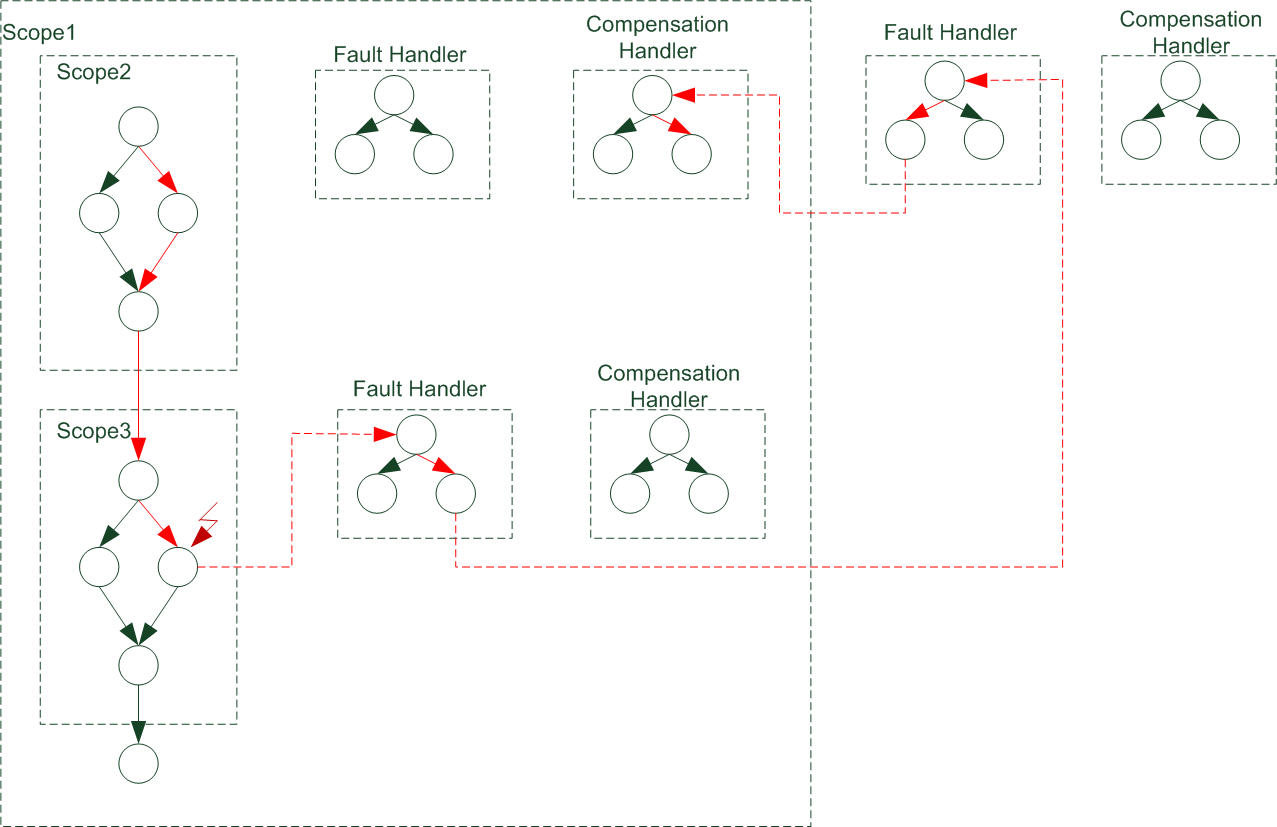
\includegraphics[width=0.9\textwidth]{bilder/Fault_Compensation.png}
		\caption{Kontrollfluss eines BPEL Prozesses}
	\label{fig:ExamlpleBPELProzess}
\end{figure}

Obwohl die Fehlererkennungsquote gegen�ber der Anweisungsabdeckung steigt, werden nicht alle Aspekte des Kontrollflusses erfasst. W�hrend jeder Zweig f�r sich alleine betrachtet wird, bleiben die Kombinationen von Zweigen unber�cksichtigt. 

In den n�chsten beiden Abschnitten werden die f�r WS-BPEL spezifischen
Testabdeckungsmetriken vorgestellt: Link- und Handlerabdeckung.      

\subsection{Link Abdeckung}
Das Link-Konzept ist in WS-BPEL ein wichtiges aber komplexes Modellierungsmittel. Die Links dienen der Synchronisation zwischen parallelen Aktivit�ten. Das Verhalten der Links kann mit Hilfe von \textit{transition} und \textbf{joinCondition} kontrolliert werden. Durch diese Bedingungen ist es m�glich komplexe Logik zu modellieren. Daraus ergibt sich die zwingende Notwendigkeit die Links und deren Verhalten zu testen. 
 
F�r die Definition einer entsprechenden Metrik wird eine Auswertungsfunktion
definiert). Let $f$ be a boolean function (or propositional statement),
$Var(f)$ yields all the propositional variables used in $f$ . Let $F$ be a set
of boolean functions and $B$ be the boolean set (true, false), a variable
assignment of $F$ is a mapping $assign: Var(F)\rightarrow B$, and the set of
all possible variable assignments of $F$ is denoted by $Assign(F)$. An
evaluation function is a mapping $eval: F \times Assign(F)\rightarrow B$
(\cite{Ouyang2005}).

F�r die Tests sind nur die Links relevant, deren transition condition nicht mit
einem konstanten Wert belegt sind, sondern mit einem Ausdruck, der erst zur
Laufzeit ausgewertet werden kann. Es ist dabei wichtig, dass der Ausdruck
sowohl zu $true$ als auch zu $false$ ausgewertet wird, um das Verhalten in beiden F�llen zu testen.

Die entsprechende Metrik hei�t $Link\ Coverage$ und wird wie folgt definiert:
\begin{itemize}
	\item $l \in_{\pi 2}\mathcal{LR}$,
	\item $f=transcon(l)$,
	\item $Assign_{test}\subseteq Assign(f)$ die Menge der Kombinationen von Variablenbelegungen, die beim Testen stattgefunden sind,
\end{itemize}
\begin{equation*}
\begin{split}
\mathcal{L}=\frac{\{\left|l\in_{\pi 2}\mathcal{LR}|Var(f)\neq \emptyset\wedge eval(f,Assign_{test}(Var(f))=true)\right|
}{2*\left|\{l\in_{\pi 2}\mathcal{LR}|Var(f)\neq \emptyset \}\right|}+
\\\frac{\{\left|l\in_{\pi 2}\mathcal{LR}|Var(f)\neq \emptyset\wedge eval(f,Assign_{test}(Var(f))=false)\right|\}}{2*\left|\{l\in_{\pi 2}\mathcal{LR}|Var(f)\neq \emptyset \}\right|}
\end{split}
\end{equation*}
	Damit es m�glich ist, die 100\%  Abdeckung dieser Metrik zu erreichen, werden nur die Links ber�cksichtigt, derenn transition condition mindestenns eine Variable enth�lt ($Var(f)\neq \emptyset$).
	
	Au�erdem ist es wichtig, dass nur die Links beachtet werden, deren transition condition beim Testen ausgewertet wurde und nicht durch $DPE$ auf $false$ gesetzt wurde. Anderenfalls k�nnen sehr einfache Tests, die die zugeh�rige Logik nicht testen, sehr schnell 50\% Abdeckung dieser Metrik erreichen. So eine Metrik w�rde dem Verh�ltnis zwischen Abdeckung und Testqualit�t (siehe Abschnitt ) widersprechen.

\subsection{Fault und Compensation Handler Abdeckung}
WS-BPEL Sprache hat ein Konzept zur strukturierten Behandlung von
Laufzeitfehlern. Die Umschaltung von normalen auf \textit{FaultHandler-}Kontrollfluss erfolgt automatisch beim Auftreten eines Fehlers. Was nichts anderes hei�t, als dass der zugeh�rige \textit{FaultHandler} ausgef�hrt wird. Die Fehler k�nnen auch in den \textit{Compensation} und in den \textit{FaultHandler} selbst auftreten. Die Tatsache, dass die
BPEL-Prozesse langlebig sein k�nnen und in unternehmenskritische Bereichen eingesetzt werden, verdeutlicht die Notwendigkeit, das Verhalten des Systems auch im
Fehlerfall umfassend zu testen. Demzufolge sollten die entsprechenden Handler durch die Tests abgedeckt werden. Die in diesem Abschnitt vorgestellten Metriken
k�nnen dabei als Indikator f�r die Testqualit�t bez�glich der Fehlerbehandlung und Kompensation dienen.

\textbf{FaultHandler.} Eine wichtige Information beim Testen des Systems im
Fehlerfall ist, ob alle  $catch$- bzw $catchAll$-Bl�cken durch die Tests
ausgef�hrt werden.   

\begin{itemize}
	\item $A_{catch}=\{a\in \mathcal{A}^{structured}\cup \mathcal{A}^{basic}|(s,f,a)\in \mathcal{HR}\wedge f\in \mathcal{E}_{fault}\wedge s\in \mathcal{A}_{scope}\}$ die Menge der top-level Aktivit�ten in allen $catch$- und $catchAll$-Bl�cken, 
	\item $\left|A_{catch}\right|$ entspricht der Anzahl von catch- und catchall-Bl�cken
	\item $A^{executed}_{catch}=\{a\in A_{catch}|\exists (s,f,a)\in \mathcal{HR}\wedge branch\_executed((s,f,x))=true\}$ die Teilmenge der Aktivit�ten aus $A_{catch}$, die getestet wurden,
\end{itemize}
\[
FH=\frac{\left|A_{catch}\right|}{\left|A^{executed}_{catch}\right|}
\]

Im Rahmen einer Fehlerbehandlung ist es m�glich, die
eigentlich in sich erfolgreichen Aktionen r�ckg�ngig zu machen. Daf�r sind in
WS-BPEL die Compensation Handler vorgesehen.
\textbf{Compensation Handler.}
\begin{itemize}
	\item $A_{compensation}=\{a\in \mathcal{A}^{structured}\cup \mathcal{A}^{basic}|(s,c,a)\in \mathcal{HR}\wedge c\in \mathcal{E}_{compensate}\wedge s\in \mathcal{A}_{scope}\}$ die Menge der top-level Aktivit�ten in allen Compensation Handler
	\item $\left|A_{compensation}\right|$ entspricht der Anzahl der Compensation Handler
	\item $A^{executed}_{compensation}=\{a\in A_{compensation}|\exists (s,c,a)\in \mathcal{HR}\wedge branch\_executed((s,c,a))=true\}$ die Teilmenge der Aktivit�ten aus $A_{compensate}$, die getestet wurden,
\end{itemize}
\[
CH=\frac{\left|A^{executed}_{compensation}\right|}{\left|A_{compensation}\right|}
\]

Da die Gesch�ftsprozesse in der Regel langlebig sind und dar�ber hinaus sensitive
Daten verarbeiten k�nnen, ist eine ausreichende Fehlerbehandlung zwingend notwendig.
Im Rahmen einer Fehlerbehandlung ist oft das Zur�cksetzen vorangegangener �nderungen erw�nscht. Daf�r sind CompensationHandler in BPEL vorgesehen, die das R�ckg�ngig-machen von eigentlich in sich erfolgreichen Aktionen �bernehmen.

Aufgrund dieser besonderen Wichtigkeit der Fehlerbehandlung muss das Verhalten des Systems im Fehlerfall umfassend getestet werden. Die in diesem Abschnitt vorgestellten Metriken k�nnen dabei als Indikator f�r die Testqualit�t bez�glich der Fehlerbehandlung und Kompensation dienen.
 
\textbf{FaultHandler.}
Eine wichtige Information ist zum Beispiel, ob alle durch den Programmierer vogesehen Fehlerbehandlungen in Form von \textit{catch}- bzw \textit{catchAll}-Bl�cken durch die Tests stimuliert werden. 
Die folgende Definition legt die dazugeh�rige Metrik fest: 
\[
	FaultHandlerAbdeckung=\frac{\text{Anzahl der getesten \textit{catch}- und \textit{catchAll}-Bl�cken }}{\text{Anzahl der \textit{catch}- und \textit{catchAll}-Bl�cken}}
\]

Die impliziten \textit{FaultHandler} werden nicht ber�cksichtigt. Die sogenannten \textit{Inline-FaultHandler}, die direkt in die \textit{invok}e-Aktivit�ten integriert sind, m�ssen dagegen in die Berechnung einflie�en.

\textbf{Compensation Handler.}
Diese Metrik gibt den Abdeckungsgrad der \textit{CompensationHandler} an: 
\[
	CompensateHandlerAbdeckung=\frac{\text{Anzahl der getesten \textit{CompensationHandler}}}{\text{Anzahl der \textit{CompensationHandler}}}
\]
Die \textit{Inline-CompensateHandler} werden ebenfalls ber�cksichtigt. \\
\\





\section{Verfahren f�r die Messung der Testabdeckung}

In diesem Abschnitt werden einige Ans�tze f�r die Messung der Testabdeckung in BPEL-Prozessen betrachtet und bewertet. Zum Schluss wird eine geeignete L�sung f�r die Integration in BPELUnit-Framework ausgew�hlt.  


Die Verfahren, die in konventionellen Sprachen f�r die Messung der Abdeckung verwendet werden, k�nnen nicht direkt auf BPEL �bertragen werden. Es m�ssen einige BPEL-spezifische Restriktionen beachtet werden:
\begin{itemize}
\item BPEL-Prozesse werden in speziellen Ablaufumgebungen (\textit{BPEL-Engine}) ausgef�hrt.
\item BPEL-Prozesse k�nnen nur mit Web Services (\textit{partner}) kommunizieren.
\item Gesch�ftslogik wird in BPEL-Prozessen durch Aktivit�ten realisiert. 
\end{itemize} 


Es gibt mehrere M�glichkeiten die Informationen �ber Ablauf eines BPEL-Prozesses zu sammeln: 
\begin{itemize} 
	\item \textbf{Instrumentierung}. Der Quellcode wird vor dem Deployen und Ausf�hren modifiziert, indem bestimmte Aktivit�ten hinzugef�gt werden, die die Ausf�hrung der entsprechenden Codebereichen signalisiereb. 
	\item \textbf{Tracing}. Der Ablauf des Programms wird �ber eine Debug-API der Ablaufumgebung  mitverfolgt.
	\item \textbf{Web Service-Mock's}(\cite{Mayer2006}). W�hrend der Ausf�hrung k�nnen aufgerufene Mock-Partner (Web Services, die durch Mock's ersetzt wurden) ihre Interaktionen mit dem BPEL-Prozess protokollieren. 
	\item \textbf{Log-Dateien der BPEL-Ausf�hrungsumgebung}(\cite{Li2005}). Aus den Log-Dateien der Ausf�hrungsumgebung kann Information �ber den Ablauf des BPEL-Prozesses extrahiert werden. 
\end{itemize}

    
Die dritte und vierte M�glichkeit eignen sich f�r die Messung der Abdeckung nicht werden daher an dieser Stelle nur ganz kurz behandelt. Durch eine Erweiterung der Logik von Web Service-Mock's ist es m�glich, die Interaktionen der Mock's mit dem BPEL-Prozess zu protokollieren. Aus dise Weise lassen sich nur Auusagen �ber externes Verhalten des Prozesses (Kommunikation mit anderen Web Services) machen. Die interne Logik und der Kontrollfluss bleiben w�hrend der Laufzeit verborgen. Zur Ermittlung von Metriken fehlen damit die Informationen �ber die Ausf�hrung des Prozesses. Die Log-Dateien der Ablaufumgebungen, wenn diese �berhaupt existieren, sind anbieterabh�ngig und nicht standardisiert, was diese M�glichkeit auch ausschlie�t. 

Der Instrumentierungs- und Tracingansatz sind als Verfahren f�r die Messung der Codeabdeckung aus dem Bereich der konventionellen Programmiersprachen bekannt. Die beiden Ans�tze wurden in der Masterarbeit von P.Dul \cite{Dul2005} im Bezug auf Programmiersprache Java detailliert untersucht und verglichen.
 
\section{Instrumentierungsansatz.}

\begin{wrapfigure}[14]{r}{6cm}
\centering%
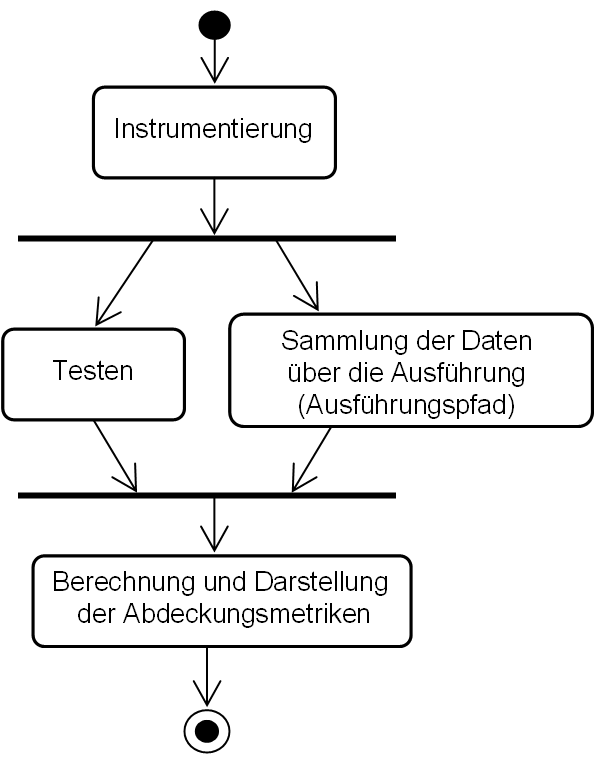
\includegraphics[width=0.3\textwidth]{bilder/Instrumentierung.png}%
\label{}
\end{wrapfigure}
Bei der Instrumentierung handelt es sich um ein einfaches Verfahren zur Messung der Testabdeckung, das in zahlreichen kommerziellen und nicht kommerziellen Werkzeugen eingesetzt wird. 
Dabei werden in den Quellcode zus�tzliche Anweisungen eingef�gt, die die Ausf�hrung bestimmter Codebereiche dokumentieren. Damit der Originalcode unver�ndert bleibt, wird die Instrumentierung auf einer Kopie durchgef�hrt. 

W�hrend der Instrumentierung werden die relevanten statistischen Daten des Quellcodes, die f�r die Auswertung der Ergebnisse notwendig sind, gesammelt und gespeichert. Anhand dieser Daten und der Information, die w�hrend der Ausf�hrung gesammelt wird, kann die Auswertung erfolgen und die Codeabdeckung ermittelt werden. Der Instrumentierungsansatz f�hrt zu einer erheblichen Vergr��erung des Programms.  

Cobertura ist ein bekanntes Werkzeug zur Ermittlung der Testabdeckung in Java-Programmen, das unter General Public License verf�gbar ist und auf dem Instrumentierungsverfahren basiert. 

..........Der Instrumentierungsansatz f�hrt offensichtlich zu einer erheblichen Zunahme der
Programmgr��e: Es wird eine Kopie des originalen Quellcodes generiert. Dann wird
die Kopie instrumentiert

\section{Tracingansatz}
Die modernen Entwicklungsumgebungen verf�gen �ber Debugger, die unter anderem eine Tracing-Funktionalit�t mit sich mitbringen.
\begin{quotation}
	\textit{Tracing bezeichnet man in der Programmierung eine Funktion zur Analyse von Fehlersuche von Programmen.
Dabei wird z.B. bei jedem Einsprung in eine Funktion, sowie bei jedem Verlassen eine Meldung ausgegeben, sodass der Programmierer mitverfolgen kann, wann und von wo welche Funktion aufgerufen wird...Wikipedia}
\end{quotation}
Diese Funktionalit�t erlaubt den Ablauf des Programms zu verfolgen und kann zur Messung der Testabdeckung genutzt werden. Auch bei diesem Ansatz wird der Quellcode im Vorfeld analysiert, um alle relevanten statischen Informationen zu sammeln. 

\section{Vergleich der Verfahren und Auswahl des Ansatzes f�r die Realisierung der Abdeckungsmessung in BPEL}
Die Tabelle \ref{Vergleichstabelle} beruht auf Ergebnissen aus \cite{Dul2005} und stellt die beiden Verfahren im BPEL-Context gegen�ber.
\begin{table}[h!]
\begin{tabular}{p{6cm}p{0.5cm}p{6cm}}
\textbf{Instrumentierungsansatz}&\ &\textbf{Tracingansatz}\\[0.1cm]
\hline \\
Basiert auf dem Hinzuf�gen von
Instrumentierungsanweisungen in
eine Kopie des zu untersuchenden
Quellcodes.&\ &
 Basiert auf den F�higkeiten des
Debuggers, Informationen
�ber das ablaufende
Programm zu erhalten.\\
\\
 Es besteht grunds�tzlich die
Gefahr den Programmablauf oder
die Programmlogik durch das
Hinzuf�gen von Instrumentierungsanweisungen zu
ver�ndern.&\ &
 Es besteht keine Gefahr, dass der
Programmablauf oder die Programmlogik
beim Tracingansatz
ver�ndert werden.\\
\\
 Es besteht grunds�tzlich die
Gefahr von Namenskonflikten
oder der Verletzung der Spezifikation.&\ &
 Es besteht keine Gefahr, dass
Namenskonflikte oder eine
Verletzung der Spezifikation
auftreten.\\
\\
 Overhead wird durch zus�tzliche
Aktivit�ten im Quellcode
generiert.&\ &
 Overhead wird durch die
Anwendung der Debug-API generiert.\\
\\
 Es ist eine aktivit�tsbasierte
Messung der Testabdeckung
m�glich.&\ &
 Es ist nur eine zeilenbasierte
Messung der Testabdeckung
m�glich.\\
\\
Die Messung bleibt unabh�ngig von 
Anbieter der Ablaufumgebung.&\ & 
Die Messung ist nur m�glich, wenn der Anbieter der Ablaufumgebung eine Tracing-Funktion unterst�tzt. Die L�sung ist anbieterspezifisch.
\end{tabular}
\caption{Vergleich der Ans�tze\cite{Dul2005}}
\label{Vergleichstabelle}
\end{table}

Zahlenm��ig weist der Tracingansatz weniger Nachteile auf. Jedoch fehlt es teilweise Unterst�tzung der BPEL-Ablaufumgebungen f�r Debugging bzw. es gibt keine Tracing-Funktionalit�t, die die Verfolgung des Ablaufs erm�glichen w�rde. Noch gr��eres Problem ist, dass diese Schnittstelle in keinster Weise standardisiert ist. Alle Nachteile des Instrumentierungsansatzes entstehen aus der Tatsache, dass die Manipulation des Quellcodes stattfindet. 

Bei der Fallstudie in der oben erw�hnten Masterarbeit wurde festgestellt, dass die Messung beim Tracingansatz wesentlich langsamer ist, als beim Instrumentierungsansatz. Diese Aussage hat aber f�r den BPEL-Prozess, der die Dienste �ber Netzwerk anspricht, keine G�ltigkeit. Der Grund daf�r ist der Netzwerkzugriff, der f�r die Kommunikation notwendig ist. Auch wenn BPELUnit-Framework die M�glichkeit anbietet, den BPEL-Prozess isoliert von den einzelnen Web Servives zu testen, werden die Mock's, die Web Services simulieren, immer noch �ber Netzwerkschicht angesprochen. Die Programmeinheit, die die Meldungen �ber Ausf�hrung bestimmter Codeteile empf�ngt, muss ebenfalls �ber Netzwerkschicht angesprochen werden. Au�erdem muss die Zeit f�r die Instrumentierung ber�cksichtigt werden. Im Kapitel \ref{chap:fallstudie} werden f�r die vorgestellten Beispiele gemessene Zeitdifferenzen angegeben. 


\textbf{Auswahl des Ansatzes f�r die Realisierung der Abdeckungsmessung in BPEL}\ \\
Da nur die ersten beiden Ans�tze (Instrumentierungs- und Tracingansatz) die Realisierung der Abdeckungsmessung f�r alle definierten Abdeckungsmetriken (siehe Abschnitt \ref{metrikdefinition}) im n�tigen Umfang erm�glichen, reduziert sich die Auswahl auf diese Beiden.

Aufgrund der vorgesehenen Integration der L�sung in das BPELUnit Framework muss bei der Auswahl des Verfahrens auf die Kompatibilit�t zum Framework und den darunterliegenden Konzepten geachtet werden.  Eine der zentralen Ziele bei der Konzeption des BPELUnit Frameworks war die Anbieterunabh�ngigkeit. In dieser Hinsicht hat man sich entschieden, den Ansatz \textit{real-life Testen} zu verwenden und damit auf die Verwendung von Debug-API zu verzichten. Das Deployment ist zwar immer noch anbieterspezifisch, die Abh�ngigkeit wurde aber mit dieser Entscheidung auf einen Minimum reduziert. 
Der Einsatz der Tracing-Funktionalit�t f�r die Messung der Testabdeckung w�rde  die Verwendung des Frameworks mit BPEL-Ablaufumgebungen ausschlie�en, die keine Traicing-Funktionalit�t unterst�tzen. Au�erdem m�sste das Framework an jede einzelne \textit{Engine} angepasst werden. Demzufolge eignet sich f�r die Messung der Abdeckung im BPELUnit Framework der Instrumentierungsansatz am Besten. 

\section{Umsetzung der Abdeckungsmessung}
\subsection{Receive Message Service}
 Ziel: m�glichst wenige Eingriffe in die Logik des Programms.
  Damit die BPEL-Datei syntaktisch korrekt bleibt, muss die Datei f�r die Instrumentierung vorbereitet werden.

  \subsection{Statementabdeckung}

  
  Alle strukturierenden Aktivit�ten (bis auf Sequence) sind so konstruiert, dass sie in ihren Komponenten genau oder maximal eine Aktivit�t erlauben. Durch das Schachtelungsprinzip k�nnen trotzdem beliebig komplexe Strukturen an diesen Stellen eingef�gt werden. Wenn an diesen Stellen nur ein Basic-Aktivit�t vorhanden ist, dann kann man nicht ohne Weiteres dahinter oder davor eine zus�tzliche Aktivit�t hinzuf�gen. Das w�rde zur Verletzung der Syntaxregeln f�hren. Also muss man vor der Instrumentierung eine umschlie�ende strukturierende Aktivit�t hinzuf�gen. Da das Logging entweder direkt davor oder danach statfinden soll, ist die Sequence-Aktivit�t gut f�r diesen Zweck geeignet. 
  
  Innerhalb der Flow-Aktivit�ten erm�glicht das Link-Konzept die Synchronisationsabh�ngigkeiten zwischen den Aktivit�tten zu definieren und durch die darauf aufbauenden Bedingungen die Ausf�hrung der Aktivit�ten zu steuern. Durch das Einf�gen der Protokollieranweisungen alleine kann eine Basic-Aktivit�t, die das Ziel eines oder meheren Links ist, nicht protokolliert werden. ...
  
  L�sung Sequence-Element um diese Aktivit�t und den Link auf die Sequence verschieben. Damit ist die richtige Protokollierung unabh�ngig vom suppressJoin-Wertes garantiert. Die Crossing-Boundary Bedingung wird durch den Eingriff auch nicht verletzt.
  
  
 
\lstset{emph={joinCondition,target }, emphstyle=\color{blue}}
      \begin{lstlisting}[caption=Beispielcode]{Name}
<flow>
  <links>
    <link name="CtoD"/>
  </links>
  <receive name="C" ...>
    <source linkName="CtoD"/>
  </receive>
  <invoke ... joinCondition=...>
    <target linkName="CtoD"/>
  </invoke>
</flow>      \end{lstlisting}

\lstset{emph={[2]sequence}, emphstyle=[2]\color{red}}
      \begin{lstlisting}[caption=Beispielcode][firstnumber=1]{Name}
<flow>
  <links>
    <link name="CtoD"/>
  </links>
  <receive name="C" ...>
    <source linkName="CtoD"/>
  </receive>
  <sequence joinCondition=...>
    <target linkName="CtoD"/>
    <!--Logging-->
    <invoke .../>
    <!--Logging-->
  </sequence>
</flow>      \end{lstlisting}


\subsection{Zweigabdeckung}

Jede Kante wird geloggt durch Einf�gen von Marken vor den Aktivit�ten

otherwise oder else einf�gen

sequenzen Einf�gen

 Flow: beim Fehler.
 
 \subsection{Fault Handler Abdeckung}

\subsection{Compensation Handler Abdeckung}
\chapter{Design und Implementierung}
Die Information �ber tats�chliche Ausf�hrung der Aktivit�ten hat einen Mehrwert gegen�ber der Information, dass eine Aktivit�t zur Ausf�hrung stimuliert wurde (aber evtl. nicht erfolgreich ausgef�hrt werden konnte). Deswegen erfolgt das Logging jeweils \textit{nach} der Ausf�hrung der entsprechenden Aktivit�t.  Die Aktivit�ten, die den normalen Kontrollfluss �ndern oder den Prozess beenden, k�nnen allerdings auf diese Weise nicht bzw. nur sehr umst�ndlich registriert werden:  
\begin{itemize}
	\item \textit{throw}
	\item \textit{rethrow}
	\item \textit{compensate}
	\item \textit{compensateScope}
	\item \textit{exit}
\end{itemize}
\textit{Exit} beendet den Prozess und kann logischerweise nur vor der Ausf�hrung erfasst werden. Die \textit{throw-}, \textit{rethrow-}, \textit{compensate-} und \textit{compensateScope-}Aktivit�ten unterbrechen den normalen Kontrollfluss und veranlassen die Ausf�hrung der entsprechenden Handler. Obwohl die tats�chliche Ausf�hrung dieser Aktivit�ten in diesen H�ndlern registriert werden k�nnte, wurde auf Grund eines gro�en zus�tzlichen Aufwands und dazu verh�ltnism��ig kleines Informationsgewinns entschieden, darauf zu verzichten und die Aktivit�ten, wie bei \textit{Exit}, vor der Ausf�hrung zu loggen. 
Aus diesem Grund werden die entsprechenden Aktivit�ten auch dann geloggt (als ausgef�hrt markiert), wenn bei der Ausf�hrung ein Fehler auftreten sollte.


Statement Ziel eines Links Also sequence drum
\section{Integration der Testabdeckungsmetriken in BPELUnit-Framework}
\section{Optimierung}
   Zusammenfassen der Marker
\chapter{Beispiele}\label{beispiele}
In diesem Abschnitt werden die Metriken an einem Besipiel demonstriert. Als Beispiel dient ein sehr einfacher BPEL-Prozess zur Verarbeitung von Bestellungen (Abbildung \ref{fig:Bespielprozess}).
\begin{figure}[htbp]
	\centering
		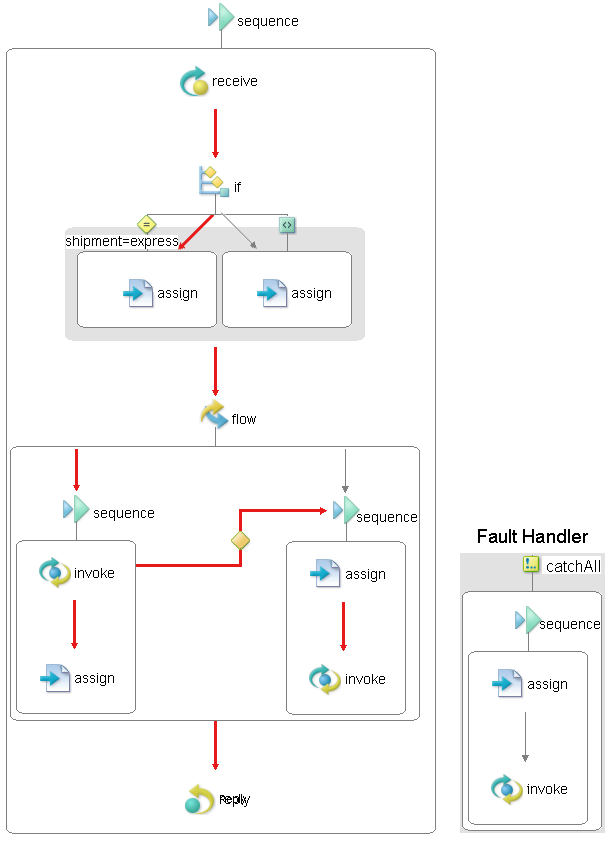
\includegraphics[width=0.6\textwidth]{bilder/Beispiel.png}
		\caption{Beispielprozess}
	\label{fig:Bespielprozess}
\end{figure}

Abh�ngig vom Liefertyp (\textit{express} oder \textit{normal}) werden die Bestellungsdaten unterschiedlich verarbeitet. Wenn der Kunde einen besonderen Status (VIP) hat, was mit dem \textit{Customer Identification}-Service festgestellt wird, dann wir der Kunde und sein Handelsvertreter �ber die Bestellung benachrichtigt.
Das wird mit Hilfe des Synchronisationslinks \textit{link\_1} modelliert, der eine explizite \textit{transition condition} aufweist: \textit{customerType='VIP'}.
F�r den Fehlerfall ist ein einfacher Fault Handler implementiert.

Der Prozess bekommt in einem Testfall eine Bestellung eines \textit{VIP}-Kunden mit folgenden Daten:
\begin{verbatim}
<order>
    <shipment>express</shipment>
    <customerId>12345</customerId>
    <productId>46298</productId>
</order>
\end{verbatim}

Es ist nur wichtig zu wissen, dass der Kunde den VIP-Status hat. Bei der Bearbeitung der Daten wird der mit roten Pfeilen markierte Pfad durchlaufen.
Mit der Erweiterung des BPELUnit-Frameworks kann die Testabdeckung ermittelt werden. Der Befehlszeilen-Client liefert die Testabdeckung im XML-Format:
\begin{verbatim}
<testingCoverage xmlns="http://www.bpelunit.org/schema/coverageResult">
  <FileStatistics filename="bpel/prozess.bpel">
    <statistic name="ActivityCoverage" totalItems="10" testedItems="7" />
    <statistic name="ActivityCoverage: assign" totalItems="5" 
                                                          testedItems="3" />
    <statistic name="ActivityCoverage: invoke" totalItems="3" 
                                                          testedItems="2" />
    <statistic name="ActivityCoverage: receive" totalItems="1" 
                                                          testedItems="1" />
    <statistic name="ActivityCoverage: reply" totalItems="1" 
                                                          testedItems="1" />
    <statistic name="BranchCoverage" totalItems="10" testedItems="8" />
    <statistic name="CompensationHandlerCoverage" totalItems="0" 
                                                          testedItems="0" />
    <statistic name="FaultHandlerCoverage" totalItems="1" testedItems="0" />
    <statistic name="LinkCoverage" totalItems="2" testedItems="1" />
    <statistic name="LinkCoverage: negativLinks" totalItems="1" 
                                                          testedItems="0" />
    <statistic name="LinkCoverage: positivLinks" totalItems="1" 
                                                          testedItems="1" />
  </FileStatistics>
</testingCoverage>
\end{verbatim}


Obwohl es sich um einen sehr einfachen BPEL-Prozess handelt, deckt ein Testfall   bereits 70\% der Basisaktivit�ten und 80\% der Zweige ab. Es wird allerding nur 50\% der Linkabdeckung erreicht und der Fault Handler wird gar nicht getestet. Der Tester kann diese Ergebnisse nutzen, um neue Testf�lle zu definieren und fehlende Bereiche abzudecken.
\chapter{Fallstudie}
\chapter{Zusammenfassung und Ausblick}
F�r BPEL-Prozesse, die meistens zu der unternehmenskritischen Software z�hlen, ist die Qualit�t der Tests sehr wichtig. Die Wahrscheinlichkeit, Fehler und M�ngel zu identifizieren, steigt mit zunehmendem Wert des Testabdeckungsma�es.

In dieser Arbeit wurden Codeabdeckungsmetriken f�r BPEL-Prozesse definiert:
\begin{itemize}
	\item Aktivit�tabdeckung: zeigt, wie viele Basisaktivit�ten bei den Tests ausgef�hrt wurden,
	\item Zweigabdeckung: zeigt, wie viele Zweige bei den Tests aktiviert wurde,
	\item Linkabdeckung: zeigt, wie viele Links bei den Tests ausgewertet wurden,
	\item Fault und Compensation Handler-Abdeckung: zeigt, wie viele Handler bei den Tests ausgel�st wurden.
\end{itemize}

Bei der Definition der Metriken wurde darauf geachtet, dass f�r jeden BPEL-Prozess 100\%-ge Abdeckung erreichbar ist. 

Implementiert wurde die Messung der Testabdeckung als Erweiterung des BPELUnit-Frame\-works. Die Instrumentierung der BPEL-Dateien und Ermittlung der Testabdeckung erfolgt automatisch und transparent w�hrend eines Testlaufs. Es kann nur suite-bezogene Testabdeckung ermittelt werden, was keine wirkliche Einschr�nkung darstellt, wenn die Teilprozesse einzeln (jeweils eine BPEL-Datei) isoliert und getestet werden. Es werden zwei Versionen der BPEL-Sprache unterst�tzt: 1.1 und 2.0. Die Erkennung erfolgt automatisch und erfordert keine zus�tzlichen Konfigurationen. Der Eclipse-Plugin und der Befehlszeilen-Client wurden entsprechend erweitert. Die beiden Clients bieten die M�glichkeit die Metriken festzulegen, diese zu konfigurieren und nach dem Testlauf die ermittelte Testabdeckung anzuzeigen.

Der n�chste logische Schritt ist die Visualisierung. Die grafische Darstellung der Testabdeckung kann den Testentwickler bei der gezielten Testerstellung besser unterst�tzen.
F�r das Erreichen der gew�nschten oder geforderter Testabdeckung ist diese Vorgehensweise viel effizienter und kann positive Auswirkungen auf die Entwicklungszeit und -Kosten haben.

Interessant w�re eine Erweiterung des BPELUnit-Frameworks, die die Ausf�hrung mehrerer Testsuites erm�glichen w�rde. Damit w�re es auch m�glich die Testabdeckung �ber mehrere \textit{Suites} zu ermitteln. 

Ein weiterer sehr interessanter Aspekt ist die Unterst�tzung der Anforderungsabdeckung f�r BPEL-Prozesse und die Definition der anforderungsbasierten (\textit{black box}-) Tesdtabdeckungsmetriken.

Die implementierte Erweiterung des BPELUnit-Frameworks bietet eine einfache M�glichkeit, die Komplexit�t des Prozesses zu berechnen. Eine entsprechende Anpassung der Definition von Komplexit�t f�r BPEL wurde in \cite{Cardoso2006} vorgeschlagen.




Die prim�re Aufgabe der Code-Coverage-Analyse liegt darin, die im Code durch Tests abgedeckten Bereiche  zu identifizieren und einige Kennzahlen der Abdeckungen zu ermitteln
(z.B. Anzahl der Durchl�ufe einer Codezeile). Daher werden bei der Code-Coverage-Analyse w�hrend der Testausf�hrung
verschiedene Messungen durchgef�hrt, die jeweils Informationen �ber eine bestimmte Art der Abdeckung sammeln. Im
Folgenden werden die wichtigsten Messmetriken bei der Code-Coverage-Analyse aufgelistet.
wieviel des zu untersuchenden Codes tats�chlichdurch die Tests ausgef�hrt wurde. Es wird auch oft der Begriff \textit{Testabdeckung} verwendet.



Anweisungs�uberdeckung wird im allgemeinen nicht als hinreichendes Kriterium
f�ur die Vollst�andigkeit eines Tests betrachtet, ihre Auswertung ergibt sich als
Nebenprodukt der Auswertung umfassenderer �Uberdeckungskriterien. Empirische
Untersuchungen zeigen eine Fehlererkennungsrate von 15\% bis unter 20\% f�ur
reine Anweisungs�uberdeckung. Sie liefert allerdings in allen Untersuchungen h�ohere
Prozents�atze als die statische Analyse des Quelltextes.
Die Kanten�uberdeckung gilt als Standard bei kontrollflussbasierten �Uberdeckungsma�en
und wird oft als Kriterium an Tests gestellt. Sie wird als leistungsf
�ahiger Test vor allem zum Auffinden von logischen Fehlern betrachtet. Untersuchungen
bez�uglich der Leistungsf�ahigkeit streuen in einem weiten Bereich von
20\% bis 70\% gefundener Fehler. Zumeist liegen die Prozents�atze im unteren Drittel
dieses Intervalls. Studien, die ebenfalls Anweisungs�uberdeckung betrachten, zeigen
f�ur Zweig�uberdeckung eine Fehlererkennungsrate, die um 50% bis 100% �uber der
der Anweisungs�uberdeckung liegt.
Bedingungs�uberdeckung findet vor allem bei Systemen mit komplexer Verarbeitungslogik
Verwendung, die in der Regel kompliziert aufgebaute Bedingungen
verwende.



D

Erfolgsquote:
..Anweisungs�berdeckungstest 18%
..Zeig�berdeckungstest 32%
..Bedingungs�berdeckungstest ?
..Pfad�berdeckungstest 65%


Beim Erstellen von Tracedaten unterscheidet man zwischen Methoden, die es erfordern
den bestehenden Source- bzw. Objektcode zu instrumentieren und Methoden,
die automatisch Traceausgaben erzeugen. Moderne Entwicklungsumgebungen bieten
meist Techniken an, um Traceausgaben ohne Sourcecode-�Anderung zu erstellen.


Die Testabdeckungsanalyse gibt an, in welchem Umfang die durchgef�hrten Tests die zu testende Software erfasst haben.



Bis jetzt wurde Instrumentierungsansatz allgemein betrachtet, ohne auf eine bestimmte Sprache einzugehen. Jetzt werden BPEL-spezifische Einschr�nkungen untersucht. Als Erstes d�rfen nur BPEL-Aktivit�ten eingef�gt werden, sonst kann der BPEL-Prozess von der BPEL-Engine nicht ausgef�hrt werden. Um Protokollierung zu realisieren, muss eine Kommunikation von der Ausf�hrungsumgebung nach au�en stattfinden. Die einzige daf�r geeignete Aktivit�t ist \textit{invoke}. Au�erdem muss ein (lokales) Web Service eingerichtet werden, der f�r das Protokollieren zust�ndig ist. Bevor zu tief in die Details eingestiegen wird, werden zuerst die anderen L�sungsm�glichkeiten vorgestellt und besprochen.	
	
	
	\begin{itemize}
\item BPEL-Prozesse werden in speziellen Ablaufumgebungen (\textit{BPEL-Engine}) ausgef�hrt.
\item BPEL-Prozesse k�nnen nur mit Web Services (\textit{partner}) kommunizieren.
\begin{itemize}
	\item Die entsprechenden WSDL-Beschreibungen sind notwendig.
	\item Die \textit{partner link types} und \textit{partner liks} m�ssen definiert werden
\end{itemize}
	\item Businesslogik wird in BPEL-Prozesse durch BPEL-Aktivit�ten (s. Abschnitt \ref{}) realisiert. 
\end{itemize}

\begin{figure}
	\centering
		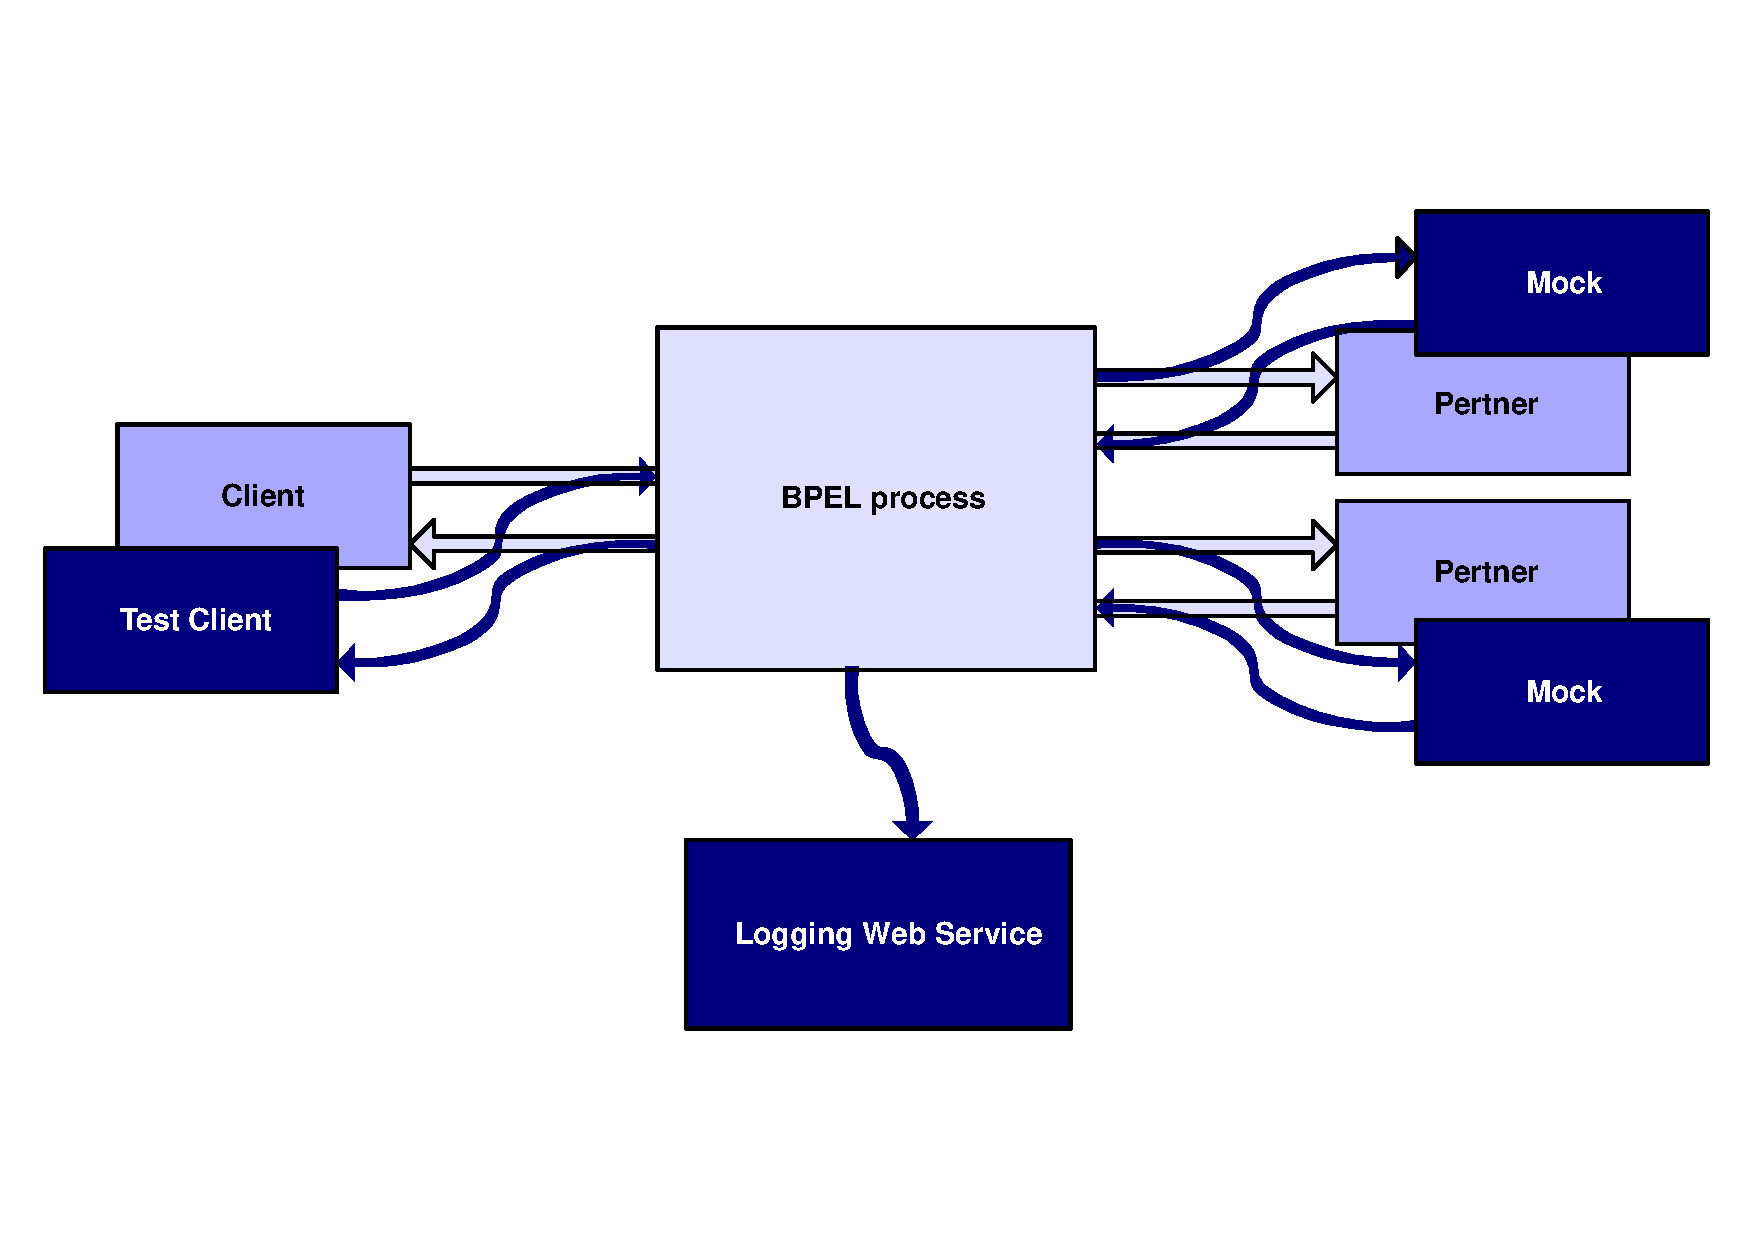
\includegraphics[width=0.90\textwidth]{bilder/loggingservice.pdf}
	\label{fig:loggingservice}
\end{figure}

\bibliographystyle{plain}
\bibliography{referenzen}
\end{document}